\documentclass{article}
\usepackage{enumitem}
\usepackage{subfigure}
\usepackage{graphicx}
\usepackage{float}
\usepackage[margin=1in]{geometry}

\begin{document}

\begin{titlepage}\centering
\vspace*{\fill}
\LARGE Instructions on Helium Source Operation
\vspace*{\fill}
\end{titlepage}

\section{Helium Source Startup Procedure}

$\bullet$ Insert tandem control power key in its place, below the low energy chain on/off button, and turn it on.\\
$\bullet$ Insert helium source control power key in its place, in the control room to the left of the labview control monitor, and turn it on.\\
$\bullet$ Check NIS and low energy tube vacuums to make sure they are what they should be (at least 10$^{-6}$ Torr).\\
$\bullet$ Check helium source filament pressure, whose gauge is found in the control room (see Fig.~\ref{figure1}). It should be around 0.04 Torr.\\
$\bullet$ Make sure the source gas valve is closed. This is a needle valve, whose switch is found in the control room to the right of helium source control power. There is a small camera in the low energy bay, which points to a mass flow meter (see Fig.~\ref{figure2}) that shows the helium flow rate in units of standard cubic centimeter per minute (sccm). If the source gas valve is closed, the flow meter should read zero sccm. A monitor in the control room is connected to that camera and also shows this flow meter. The monitor has its own remote control with which it can be turned on. Also, if it doesn not show the flow meter, check the BNC cable that is hanging from the monitor and make sure it is connected to the correct patch panel. Below the monitor, you will see many patch panels. The third patch panel from the top that has 3 rows of BNCs is the one you're looking for. It is labelled as ``TO LECAL panel''. On this patch panel, the monitor should be patched to the bottom row of input BNCs into the second input from the left side. This input is labelled as 2. Also, in the control room, below the monitor which shows extractor and attachment electrodes biases, there is a brown patch panel which is the most bottom patch panel on there. Make sure a BNC cabel is connected to the second BNC input from the left side on that patch panel. The BNC input is labelled as 2 and the actual cable that should be patched here is labelled as ``CAM 1'' and the other side of the cable goes under the floor of the control room.\\
$\bullet$ To close the gas source needle valve, lower its switch in the control room for 20 seconds and observe the flow meter on the monitor making sure it goes to zero. This action should also reduce the helium source filament pressure, whose gauge is also found in the control room (see Fig.~\ref{figure1}).\\
$\bullet$ Go to low energy bay area.\\
$\bullet$ Check to make sure both bunchers are off (see Fig.~\ref{figure3}) if you do not need the bunchers.\\
$\bullet$ Check the aperture shown on Fig.~\ref{figure4} to make sure it is out of the beam path and is grounded.\\
$\bullet$ Check the pandora slits (Fig.~\ref{figure5}) to make sure they are out all the way and are terminated.\\
$\bullet$ Open alpha source gate valve (see Fig.~\ref{figure6}) by turning the small screw found on the valve body clockwise. You need to use a screw driver for this.\\
$\bullet$ Make sure the source diffusion pump and its backing pump are on. They are both found underneath the helium source in the low energy bay area. The high vacuum gauge (see Fig.~\ref{figure7}) should be $\sim5~\times~10^{-6}$ Torr and the foreline pressure (see Fig.~\ref{figure8}) should be around 10 -- 20 mTorr. Also, the diffusion pump gate valve should be open. This can be confirmed  with a green LED light (see Fig.~\ref{figure8}) indicating the diffusion pump gate valve is open. The valve controller can be found behind the helium source panel (see Fig.~\ref{figure8}).\\
$\bullet$ Check cooling water valves (see Fig.~\ref{figure9}). The bottom 3 valves are return valves and they are always open. Very slightly move the valves to ensure they are open. The three top valves are supply valves. If you are standing besides them facing DENIS source, the far right supply valve should already be open to cool the diffusion pump. Make sure this is the case. The middle and left valves might be closed. If so, open them (by turning the valves clockwise) but not all the way. The water is very clod, and therefore these valves do not need to be opened all the way.\\
$\bullet$ Check Freon level (see Fig.~\ref{figure10}) to make sure it is between the two red marks on the Freon tube. If not, fill the Freon tube as follows:
\begin{itemize}
  \item Open the small valve with a green handle that is on a red plastic tube to the right of the Freon tube.
  \item Open the valve with a circular black handle to the left of the green valve.
  \item Fill Freon tube until the level is close to the top red mark on the tube.
  \item Close the black valve. Then, close the green valve.
\end{itemize}
$\bullet$ Turn on Freon pump, whose switch is found beside the Freon tube. Make sure Freon is flowing in its system. Is that is the case, the paddle wheel inside the Freon flow meter (see Fig.~\ref{figure10}) should be rotating continuously. Make sure this is the case.\\
$\bullet$ Turn on filament cooling fan (see Fig.~\ref{figure11}) by plugging in a big yellow plug.\\
$\bullet$ Make sure both valves on the $^{4}$He bottle are closed. Then, turn on $^{4}$He roughing pump (see Fig.~\ref{figure12}).\\
$\bullet$ Open the following valves:
\begin{itemize}
  \item V20, Valve to helium source manifold, V18, V19, V2, and V1
\end{itemize}
Wait for $\sim$5 minutes to pump on the $^{4}$He manifold. The pressure gauge shown on Fig.~\ref{figure13} should go down to 30 inches of vacuum, and the flow meter shown on Fig.~\ref{figure2} should read zero sccm.\\
$\bullet$ Close valves V18, valve to helium source manifold and V20. Then, turn off the $^{4}$He roughing pump.\\
$\bullet$ Open both valves on the $^{4}$He bottle and open valve V1. The pressure gauge shown on Fig.~\ref{figure13} should now read 5 -- 10 psi.\\
$\bullet$ Turn on the cooling oil pump by holding ``Cooling pump on'' switch (see Fig.~\ref{figure14}) for a few seconds up to a minute. Do not let go of the switch until the oil pressure (see Fig.~\ref{figure15}) reaches $\geq$ 40 psi. If you let go of the switch sooner, the cooling oil pump will turn itself off.\\
$\bullet$ Go to the control room.\\
$\bullet$ Flip Filament Or Probe Bias knob on filament. Increase filament bias slowly to 10 V. Switch the Filament Or Probe Bias knob to Probe and watch probe voltage going up slowly. Very slowly repeat this process and every time increase the filament bias slowly by 10 V until you get to 140 V on the filament and 70 V on the probe.\\
$\bullet$ Increase Source Head Magnet current slowly to 1.5 A. If you go over 2 A, a circuit breaker will switch off and you will lose power to almost all the controls in the control room and this will cause you to lose the plasma. If that happens anytime during the run, go to the low energy bay and check the back of the first cabinet after the NIS magnet. At the bottom of the cabinet close to the ground, you will see two circuit breaker switches. Make sure both are on. If one is off, turn it back on again. It is probably off because the source magnet current is too high, so lower the current to 1.5 A.\\
$\bullet$ Slowly increase filament current to 10 A.\\
$\bullet$ Raise source gas needle valve slowly to increase the gas flow read on the flow meter which is shown on a monitor by a camera (see Fig.~\ref{figure2}). Keep opening the needle valve until this flow meter reads $\sim$0.8 sccm. At this point the helium source filament pressure gauge should be around 0.2 Torr. If not, raise or lower source gas needle valve until the aforementioned pressure reads 0.2 Torr.\\
$\bullet$ Increase filament current slowly by another 10 -- 15 A. Check helium source filament pressure gauge regularly to make sure the filament is not outgassing. If the helium source filament pressure gauge is rising, the filament is outgassing, in which case reduce filament current a little bit and wait. Once the helium source filament pressure stabilizes around 0.2 Torr, increase filament current some more. Put Filament Or Probe Bias knob on the probe. Once the filament current is around 45 A or so, the probe bias starts to decrease, which means the plasma arc is struck. At this point, flip Arc/Source Head Magnet knob on Arc and watch arc current slowly rising. Once the arc is stable, the probe voltage should be less than 50 V. Increase filament current up to 60 A.\\
$\bullet$ Increase focus voltage slowly to 2 KV. If the focus ON/OFF LED light (above the focus voltage knob) is not lit green, check the back on that same panel where the knob is and make sure the circuit breaker button is on the ON position.\\
$\bullet$ Go to low energy bay.\\
$\bullet$ Turn the attachment electrode as well as extractor (see Fig.~\ref{figure16}) powers on. Push HV ON bottuns and make sure Active LED lights above the voltage knobs come on. Slowly bring the voltages up together (this is important, they should be brought up together). The attachment electrode goes to 16 kV, while the extractor electrode goes to 19 kV. Make sure they are not sparking (the leakage currents should be constant, steady and low). On these two power supplies there is a current setting knob, which should be set to 6 A for both power supplies.\\
$\bullet$ Go to the main patch panel (see Fig.~\ref{figure17a}) in the low energy bay and turn the steerers power switch to OFF position.\\
$\bullet$ Patch helium source steerers on the main patch panel in the low energy bay as follows:
\begin{itemize}
  \item Steerers 1 -- 2 should be patched to Station 5D. The patch panel is to the right side of the low energy bay entrance which is in front of the elevator. The actual helium source steerer power cable comes from the steerer right after the helium ion source and before the green helium source gate valve on the helium source beamline. This cable needs to be plugged into an outlet found close to the helium source station in the low energy bay behind the source panel (see Fig.~\ref{figure17b}). Make sure this cable is connected to the outlet labeled as Station 5D.
  \item Steerers 3 -- 4 should be patched to Station 5B. The patch panel is to the right side of the low energy bay entrance which is in front of the elevator. The actual Wender steerer cable can be found close to the ion source. It is a black cable labeles as Wender. Plug it into the power outlet behind the helium source into Station 5B outlet (see Fig.~\ref{figure17b}).
\end{itemize}
$\bullet$ Turn the steerers power switch to ON position.\\
$\bullet$ Open low energy tube gate valve.\\
$\bullet$ Go to the control room.\\
$\bullet$ Slowly change the NIS magnet setting to $\sim$74 mA.\\
$\bullet$ Turn on the sodium oven switch (see Fig.~\ref{figure18}).\\
$\bullet$ Turn the big knob beside the sodium oven switch to increase the sodium oven heater current to 1 A. Wait for 30 minutes and then increase the heater current to 2.5 A. Leave it at this current afterwards and it should take between 2 to 2.5 hours for the beam current to go up. Keep tunning the beam during this time to make sure you maximize the beam intensity while the oven is being heated.\\
$\bullet$ During this 2 hour waiting time, regularly check helium source filament pressure to make sure it is around 0.2 Torr. You may need to adjust the source gas needle valve to reach 0.2 Torr on the filament pressure gauge. Also make sure the attachment and extractor electrodes are not sparking. If so, lower filament current a bit (if you decrease it too much, the arc goes out). After sparking goes away, slowly increase the filament current again.\\
$\bullet$ Beam current on low energy cup will go up slowly. You can tune it using NIS magnet, focus electrode, steerers 1 to 3, filament current, source head magnet current and Einzel lens.\\
$\bullet$ Once the beam intensity on low energy cup is around 2 $\mu$A and is more or less constant, cool down the sodium oven by opening the cooling air valve (see Fig.~\ref{figure19}) for 2 -- 3 seconds and then close the cooling air valve. If the beam intensity has dropped immediately, the oven temperature is either perfect or it might be a bit low. If the beam intensity goes up after opening the cooling air valve, then the oven is too hot and you need to reduce the oven heater current.\\
$\bullet$ Once the oven is hot enough and the beam current on low energy cup is steady, you can switch to $^{3}$He if necessary.

\begin{figure}
\begin{center}
\includegraphics[width=0.5\textwidth]{IMG_0381}\\
\end{center}
\caption{\label{figure1}Helium source filament pressure gauge found in the control room.}
\end{figure}

\begin{figure}
\begin{center}
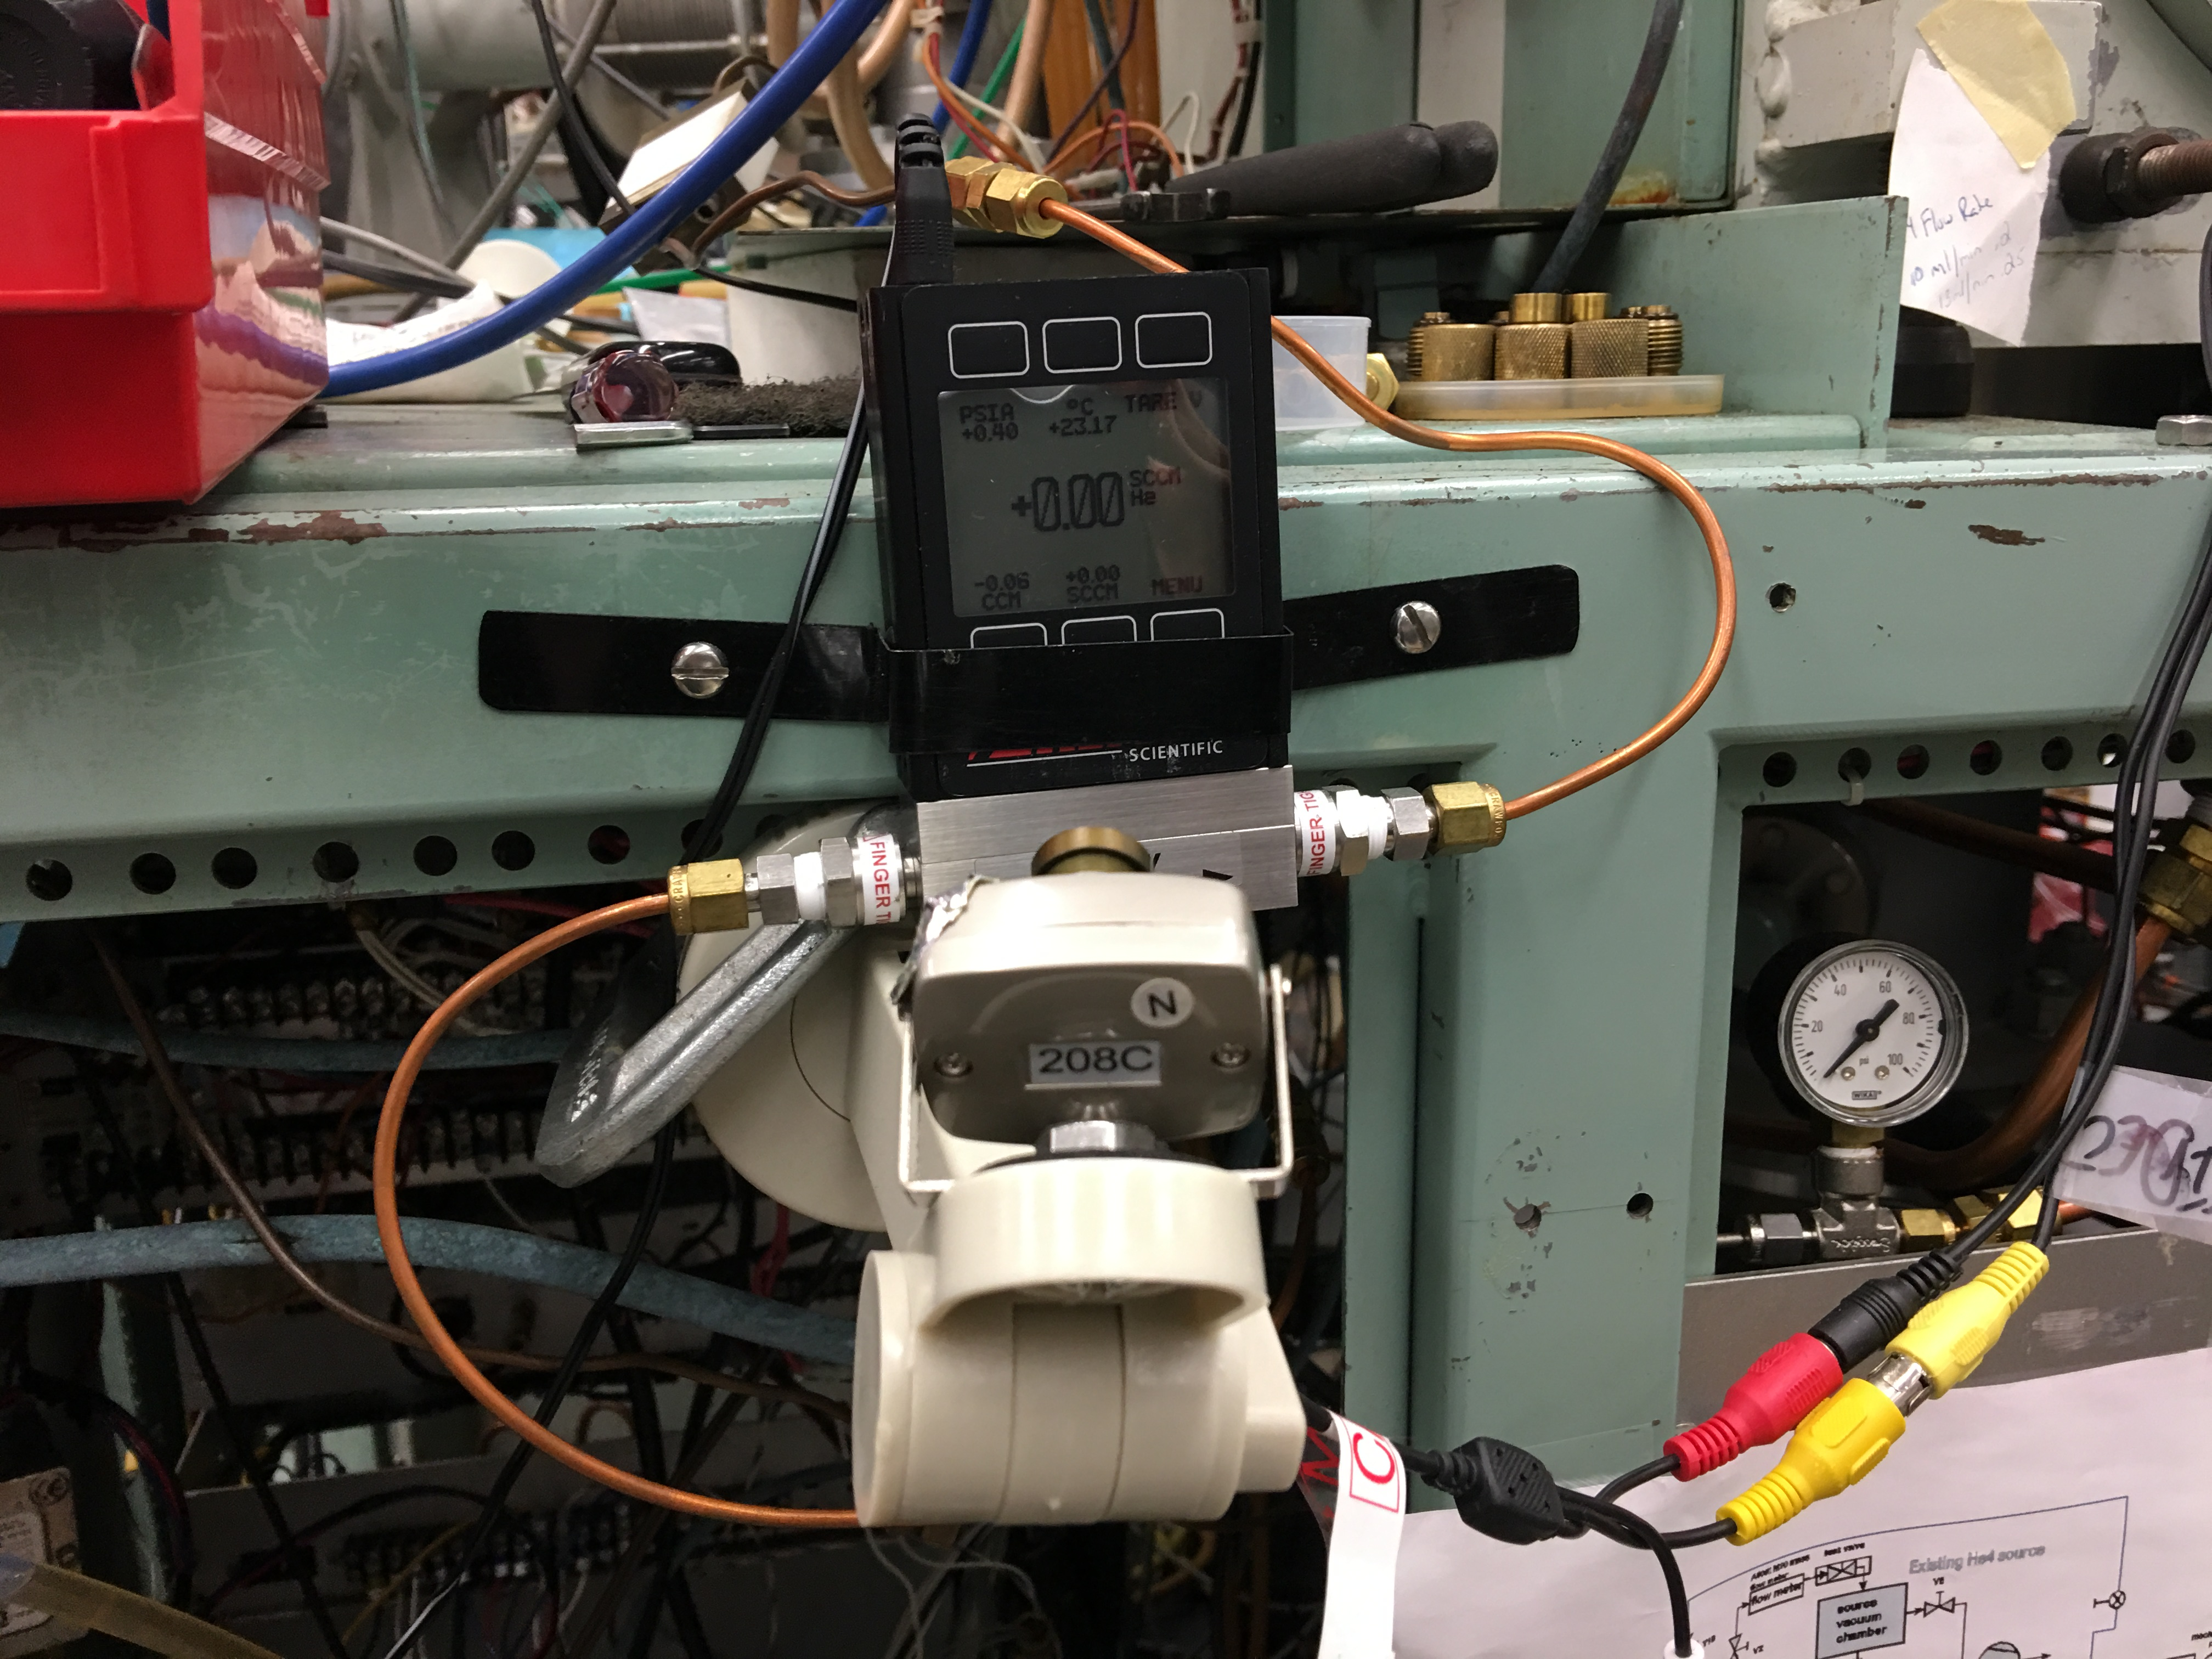
\includegraphics[width=0.5\textwidth]{IMG_0380}\\
\end{center}
\caption{\label{figure2}Helium mass flow meter (in units of standard cubic centimeter per minute) controlled by source gas needle valve. The flow meter is located in the low energy bay, and a camera projects the reading of this meter onto a monitor in the control room.}
\end{figure}

\begin{figure}
\begin{center}
  \subfigure[First chopper/buncher control panel.]{%
    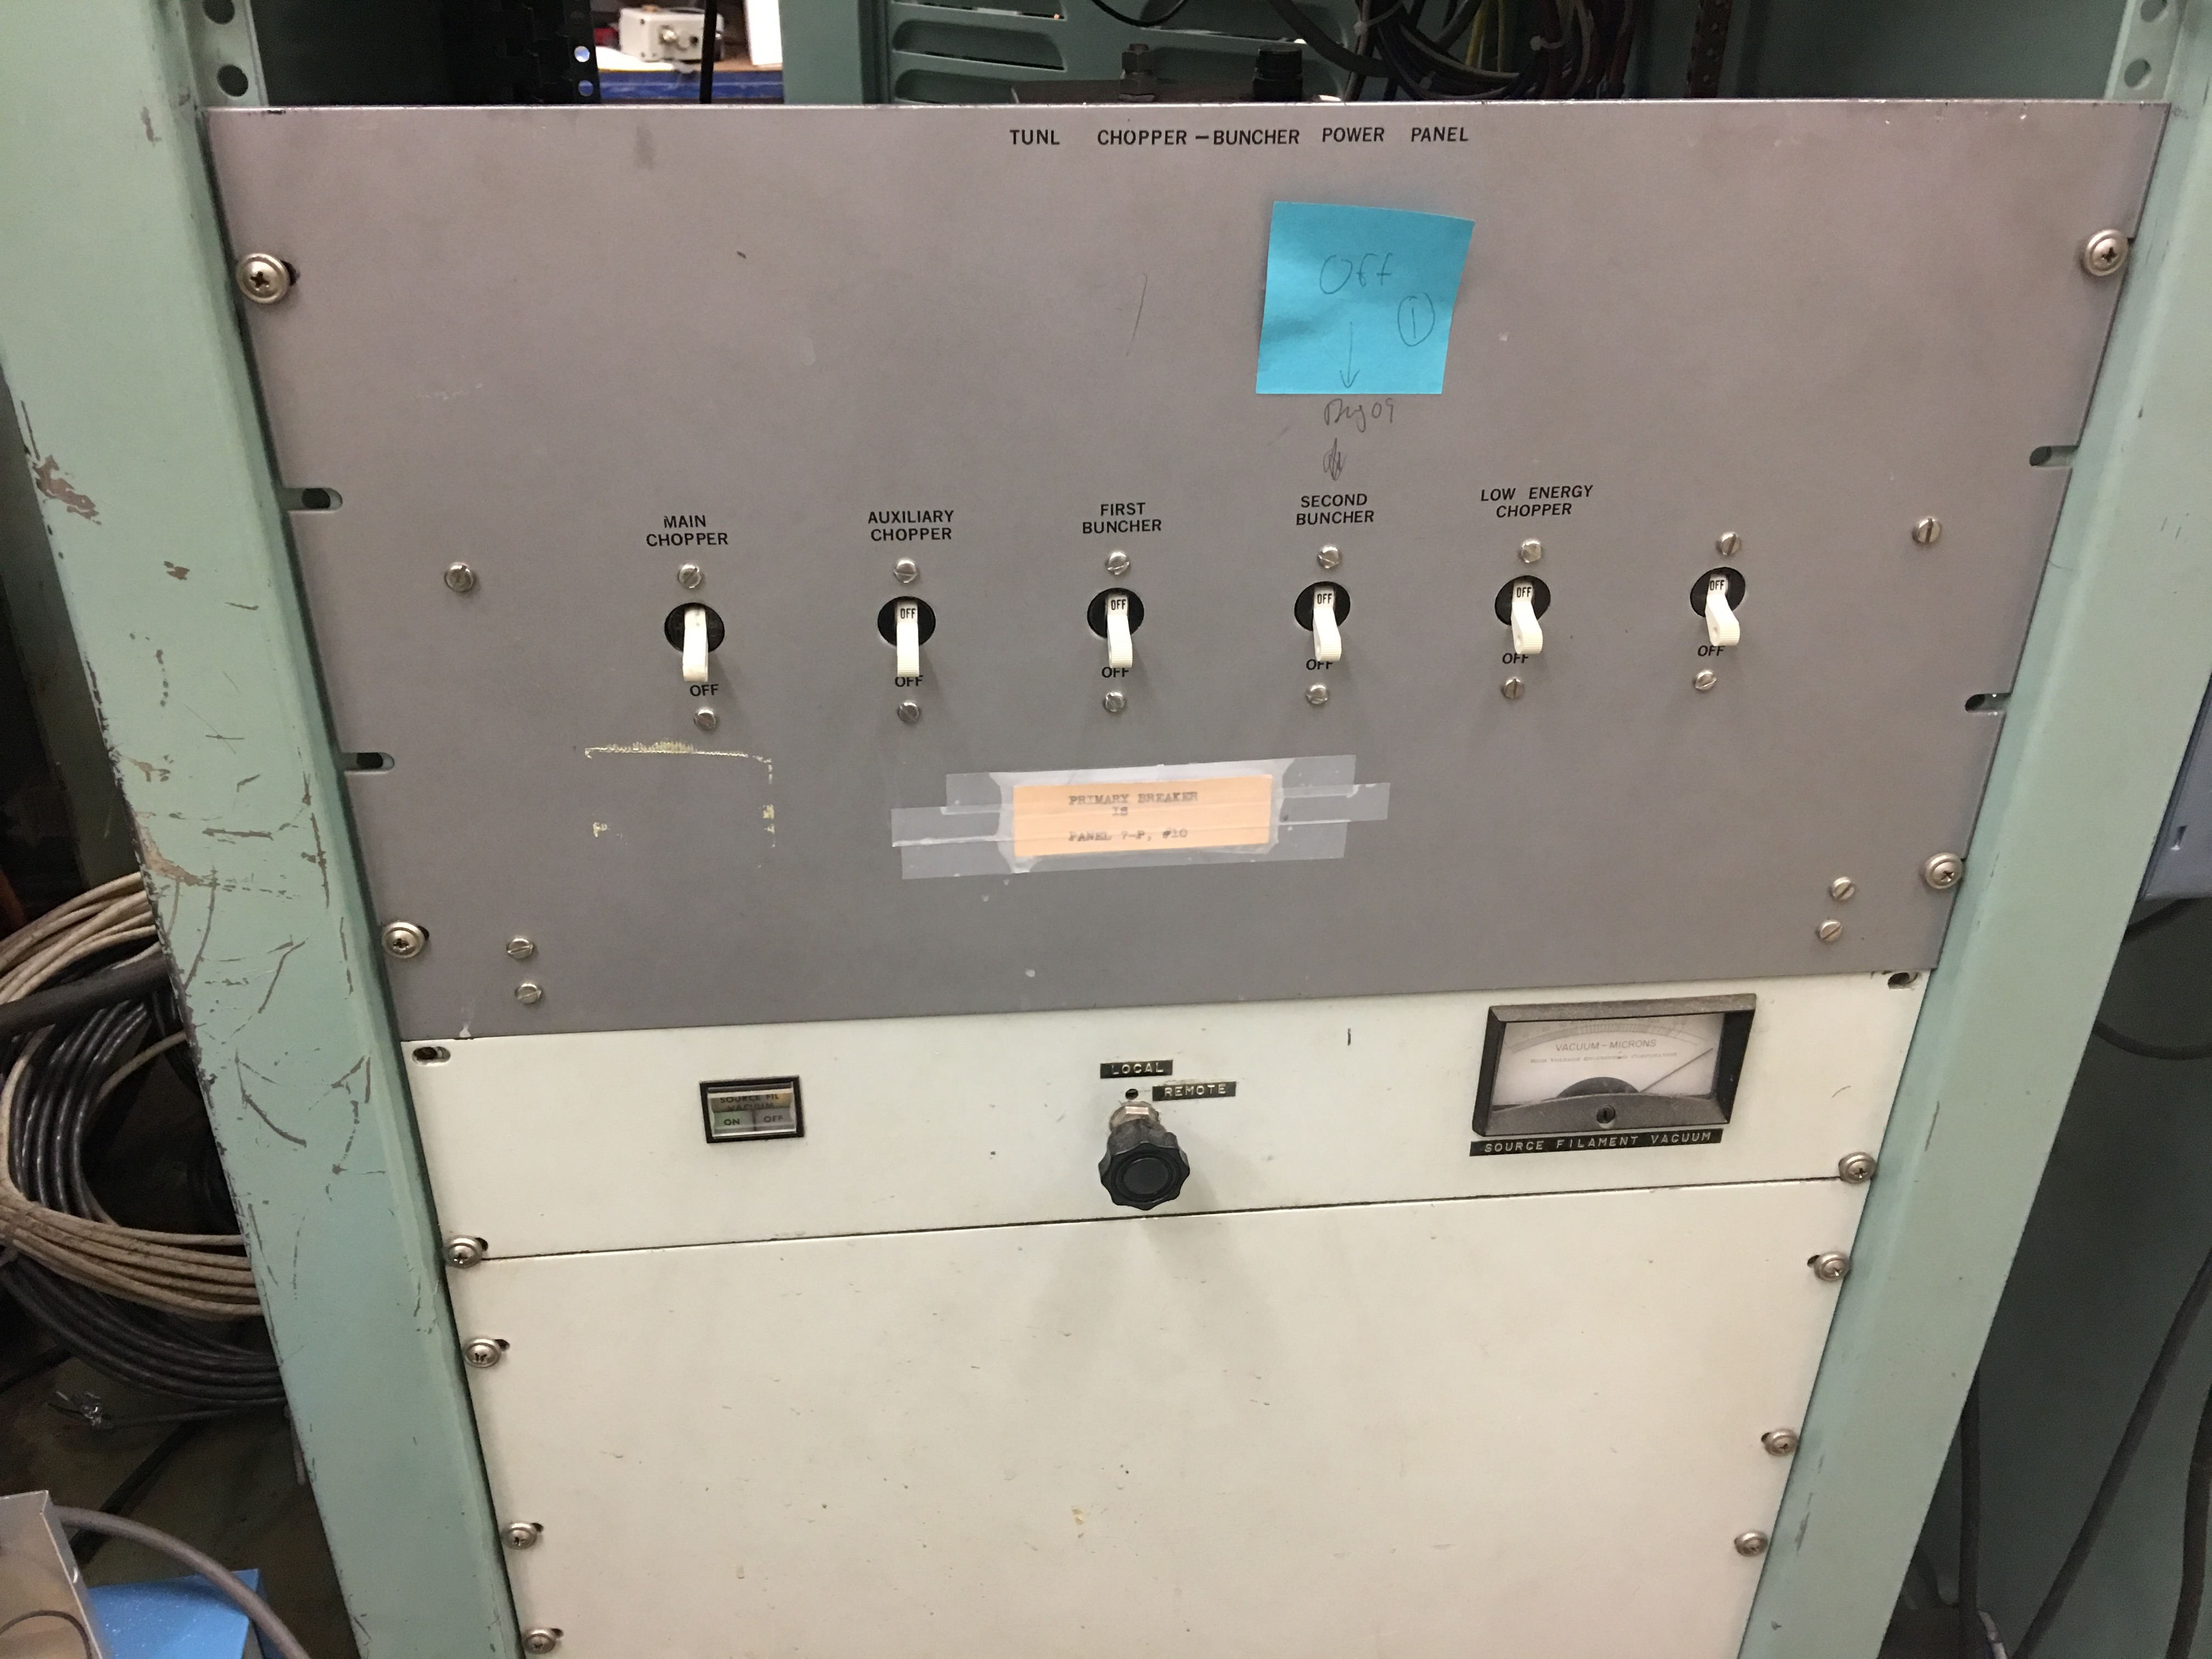
\includegraphics[width=.4\textwidth]{IMG_0442} \label{figure3a}
  }
  \quad
  \subfigure[Second chopper/buncher control panel.]{%
    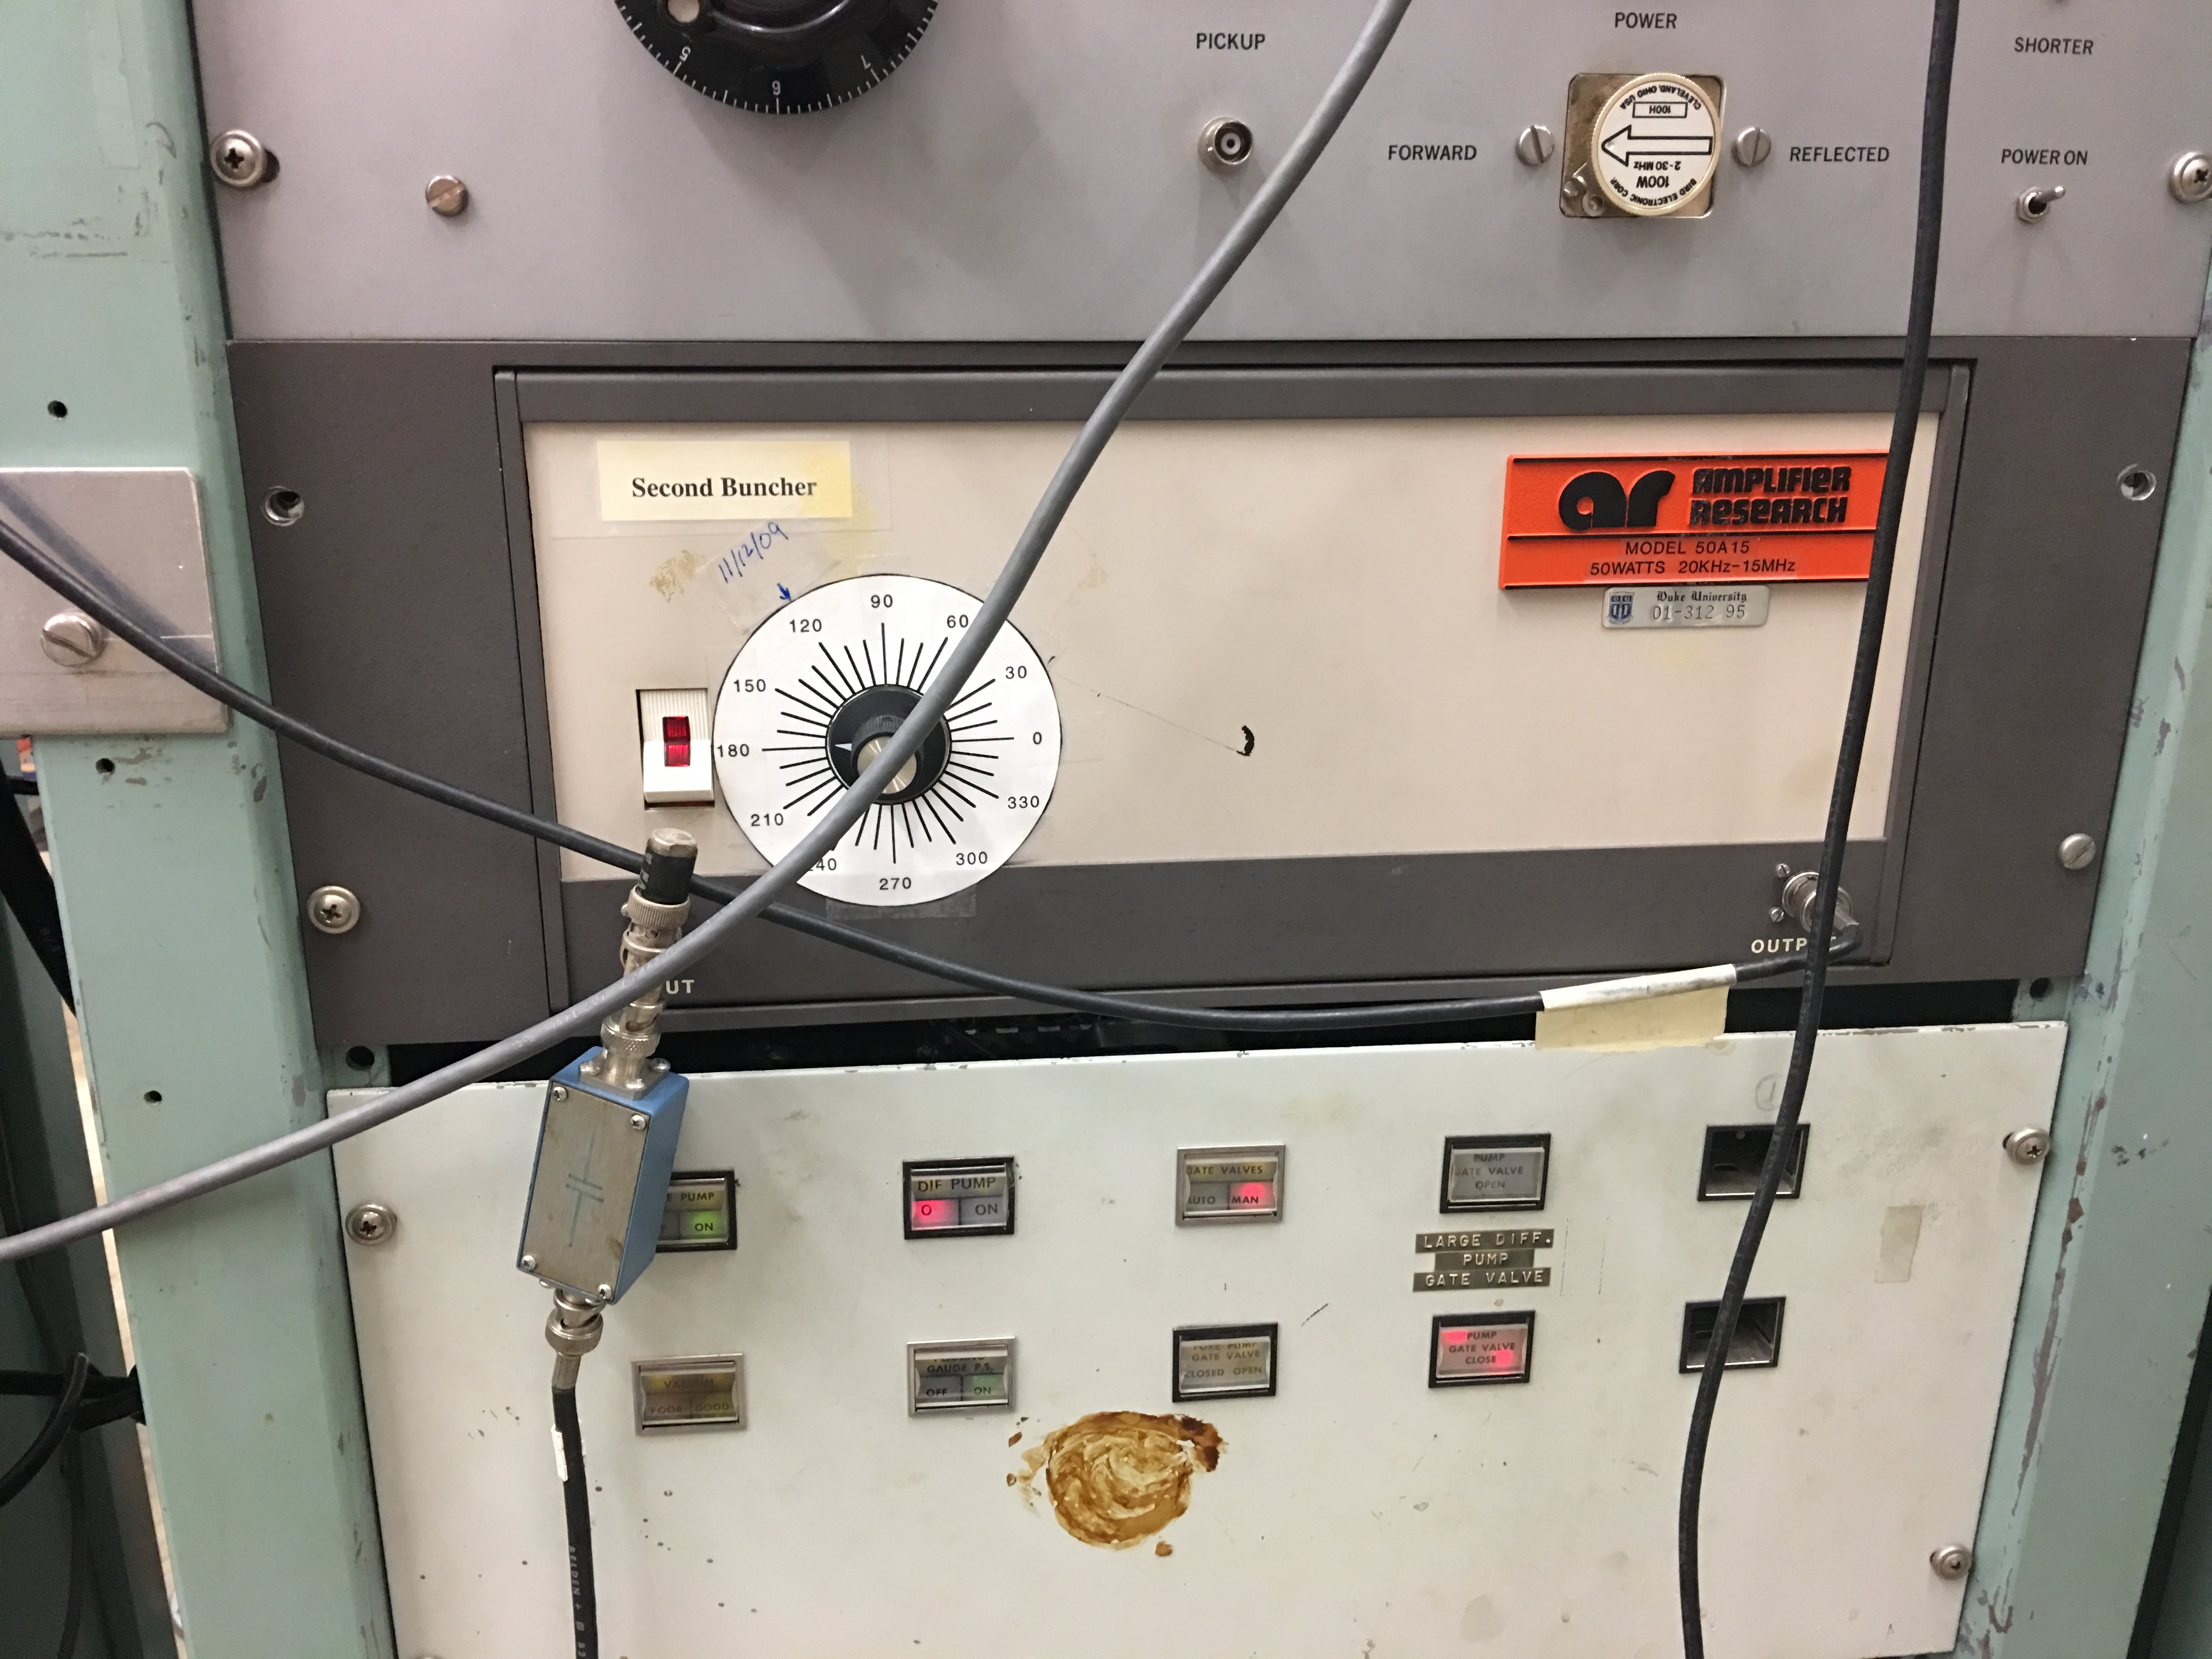
\includegraphics[width=.4\textwidth]{IMG_0443} \label{figure3b}
  }
\end{center}
  \caption{\label{figure3}Beam bunchers' control panels found in the low energy bay upstream of the tandem. You need to make sure that both of these bunchers are turned off if not in use.}
\end{figure}

\begin{figure}
\begin{center}
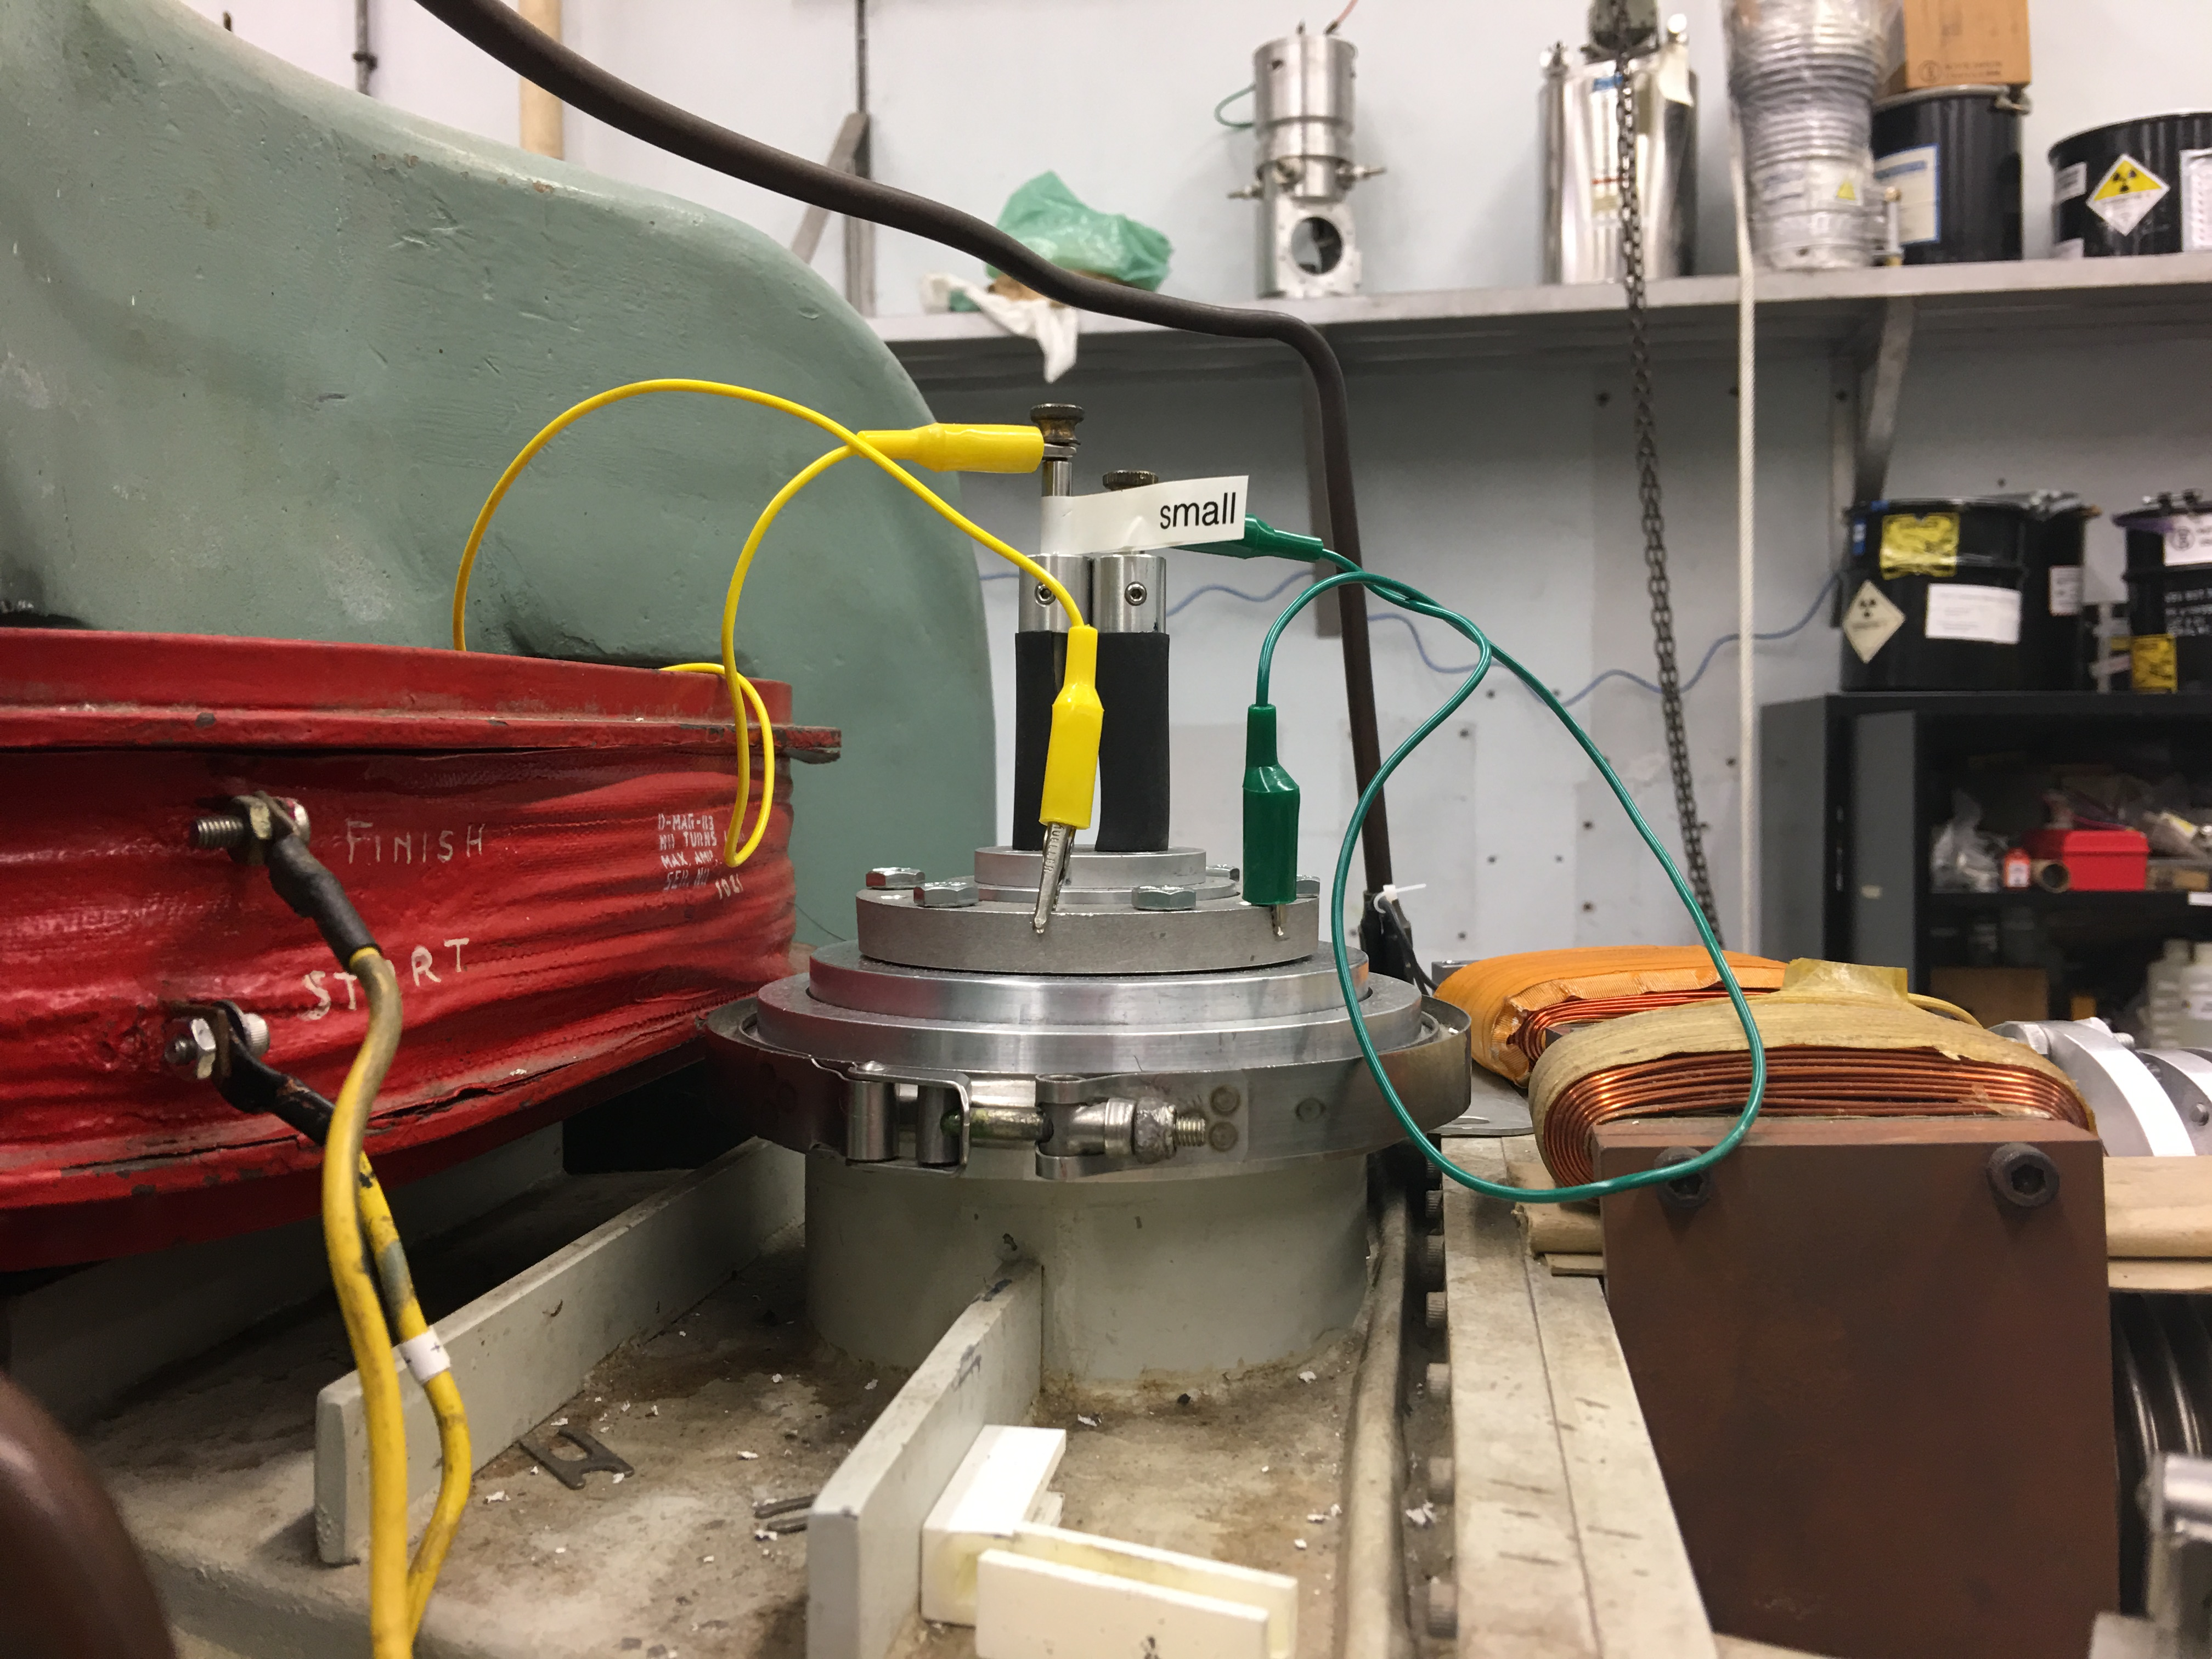
\includegraphics[width=0.5\textwidth]{IMG_0444}\\
\end{center}
\caption{\label{figure4}An aperture which should be taken out of the beam path and grounded if not used. It is found right after the NIS magnet. To take it out, simply pull the two handles up and put the two associated black spacers on them to keep them out of the beam path. To ground them, connect the aperture handles to the beamline using alligator clips.}
\end{figure}

\begin{figure}
\begin{center}
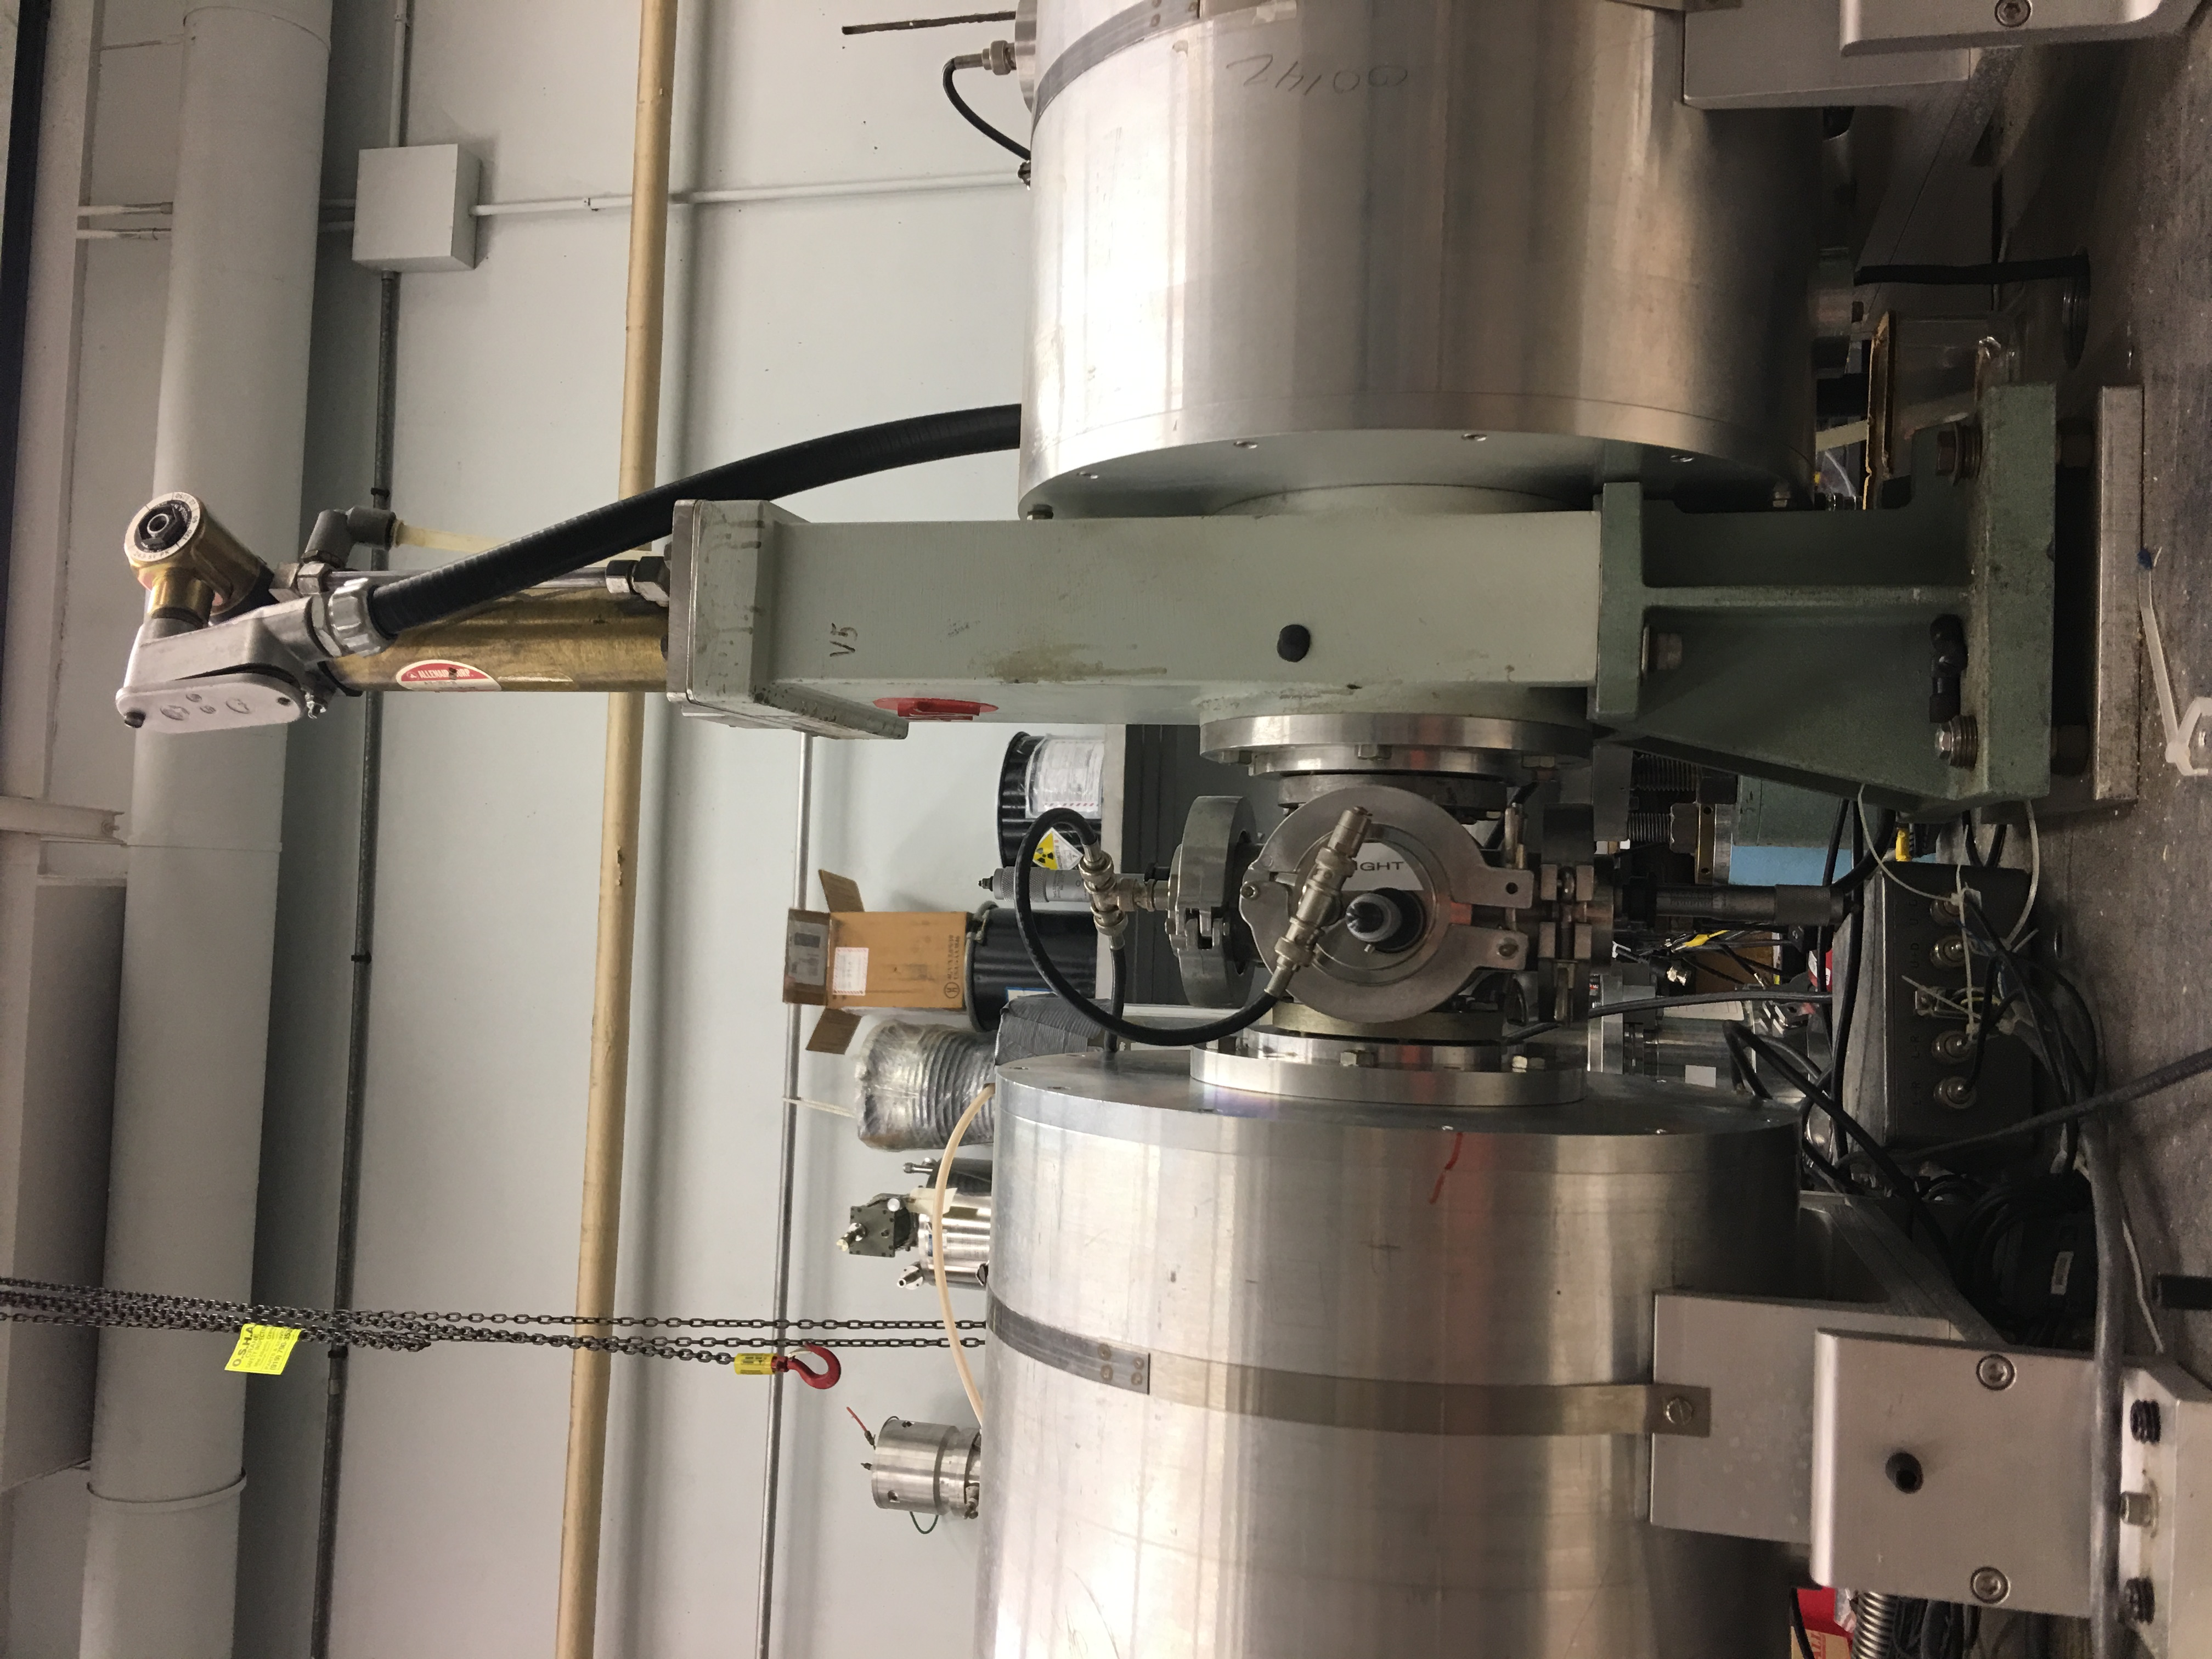
\includegraphics[width=0.5\textwidth,angle=270]{IMG_0445}\\
\end{center}
\caption{\label{figure5}Pandora slits which are usually all the way out of the beam path and are summed and terminated. They are located on the low energy beamline between the two bunchers and upstream of the low energy tube gate valve.}
\end{figure}

\begin{figure}
\begin{center}
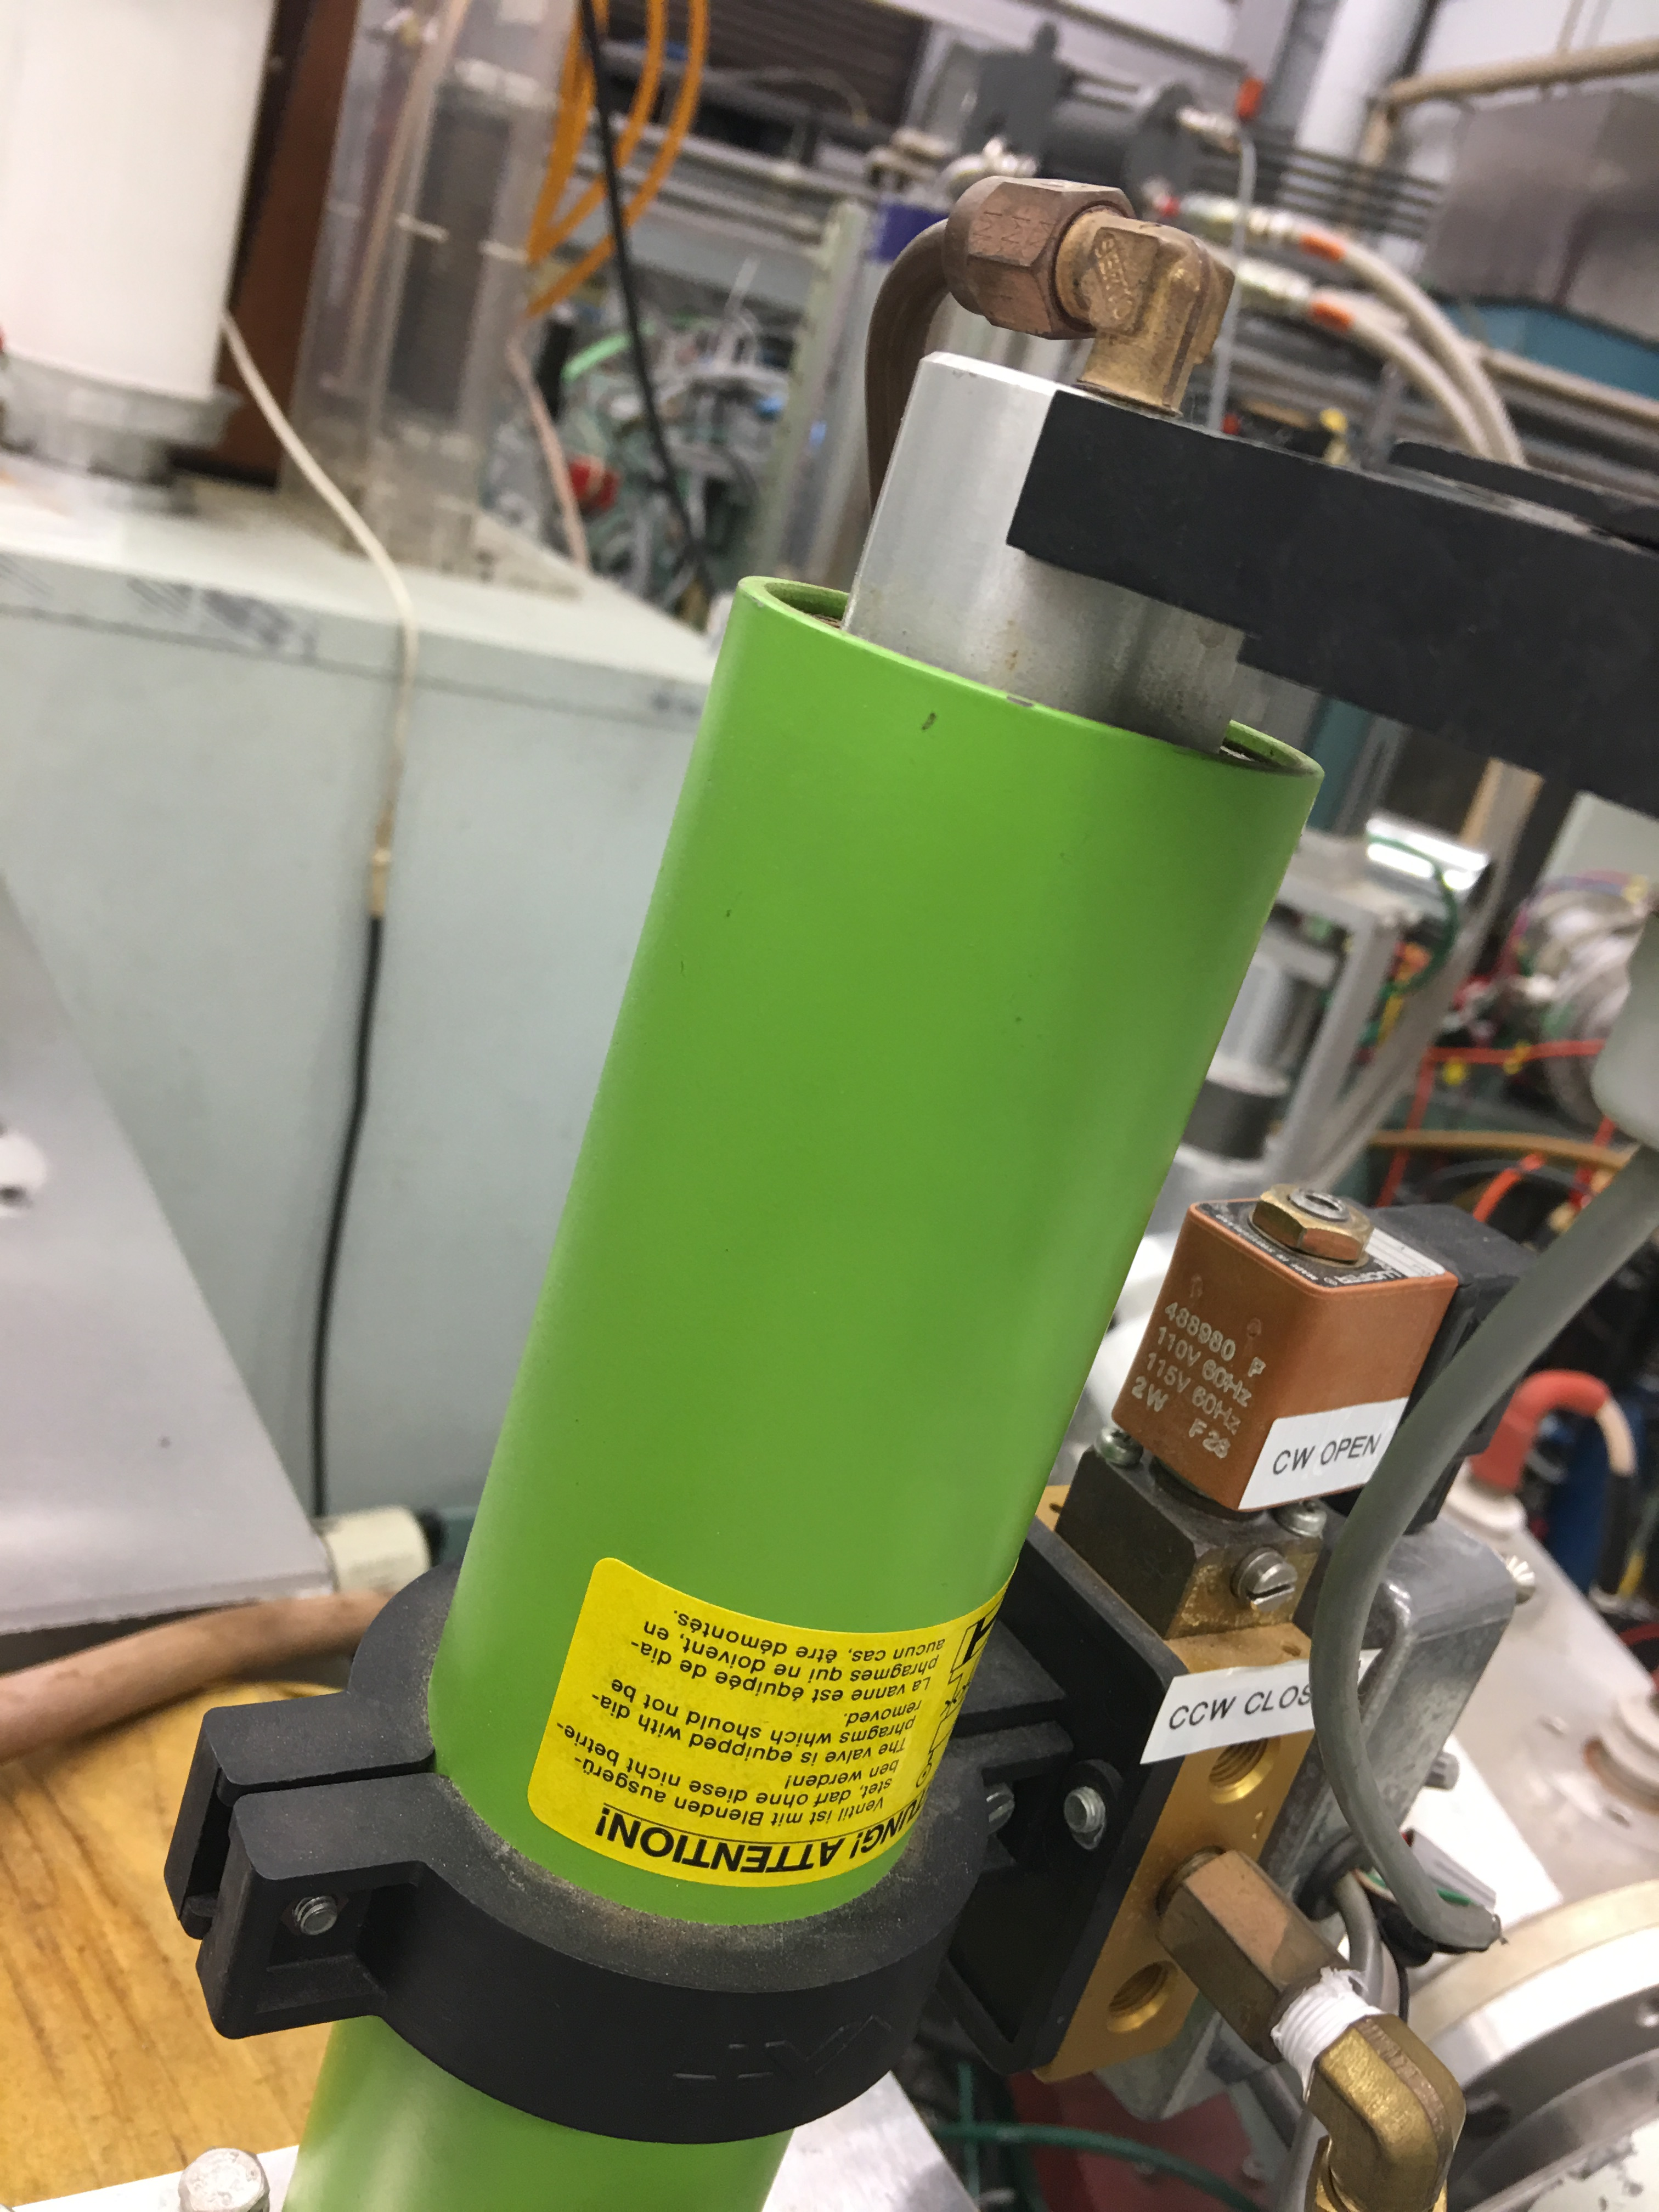
\includegraphics[width=0.5\textwidth]{IMG_0383}\\
\end{center}
\caption{\label{figure6}Alpha source gate valve in the low energy bay upstream the NIS magnet. The screw on the body of the valve can be turned clockwise to open and counter clockwise to close this valve.}
\end{figure}

\begin{figure}
\begin{center}
\includegraphics[width=0.5\textwidth]{IMG_0397}\\
\end{center}
\caption{\label{figure7}High vacuum gauge found along the helium source beamline, which should read $\sim~5~\times~10^{-6}$ Torr if the alpha source diffusion pump is on and its gate valve is open. If the device is on standby, push the far left purple button and it will come on.}
\end{figure}

\begin{figure}
\begin{center}
\includegraphics[width=0.5\textwidth]{IMG_0400}\\
\end{center}
\caption{\label{figure8}The meter to the left of the image shows the foreline pressure gauge for the diffusion pump. It is found in the low energy bay behind the alpha source panel. If the foreline pressure goes above the red indicator on the gauge, an interlock will shut down the diffusion pump, as well as the probe/filament, source magnet and focus power supplies and it will cause the plasma to be put out. To avoid this, the gas input must not be high enough to increase the foreline pressure too much. Also, sometimes unplugging the associated thermocouple gauge found beside the alpha source diffusion pump and plugging it back fixes this issue with interlock. The diffusion pump's gate valve open/close switches are also found in the same panel. Once the foreline pressure is returned to a normal value below the red indicator on this gauge, everything that was shut down by the interlock will be turned on again automatically.}
\end{figure}

\begin{figure}
\begin{center}
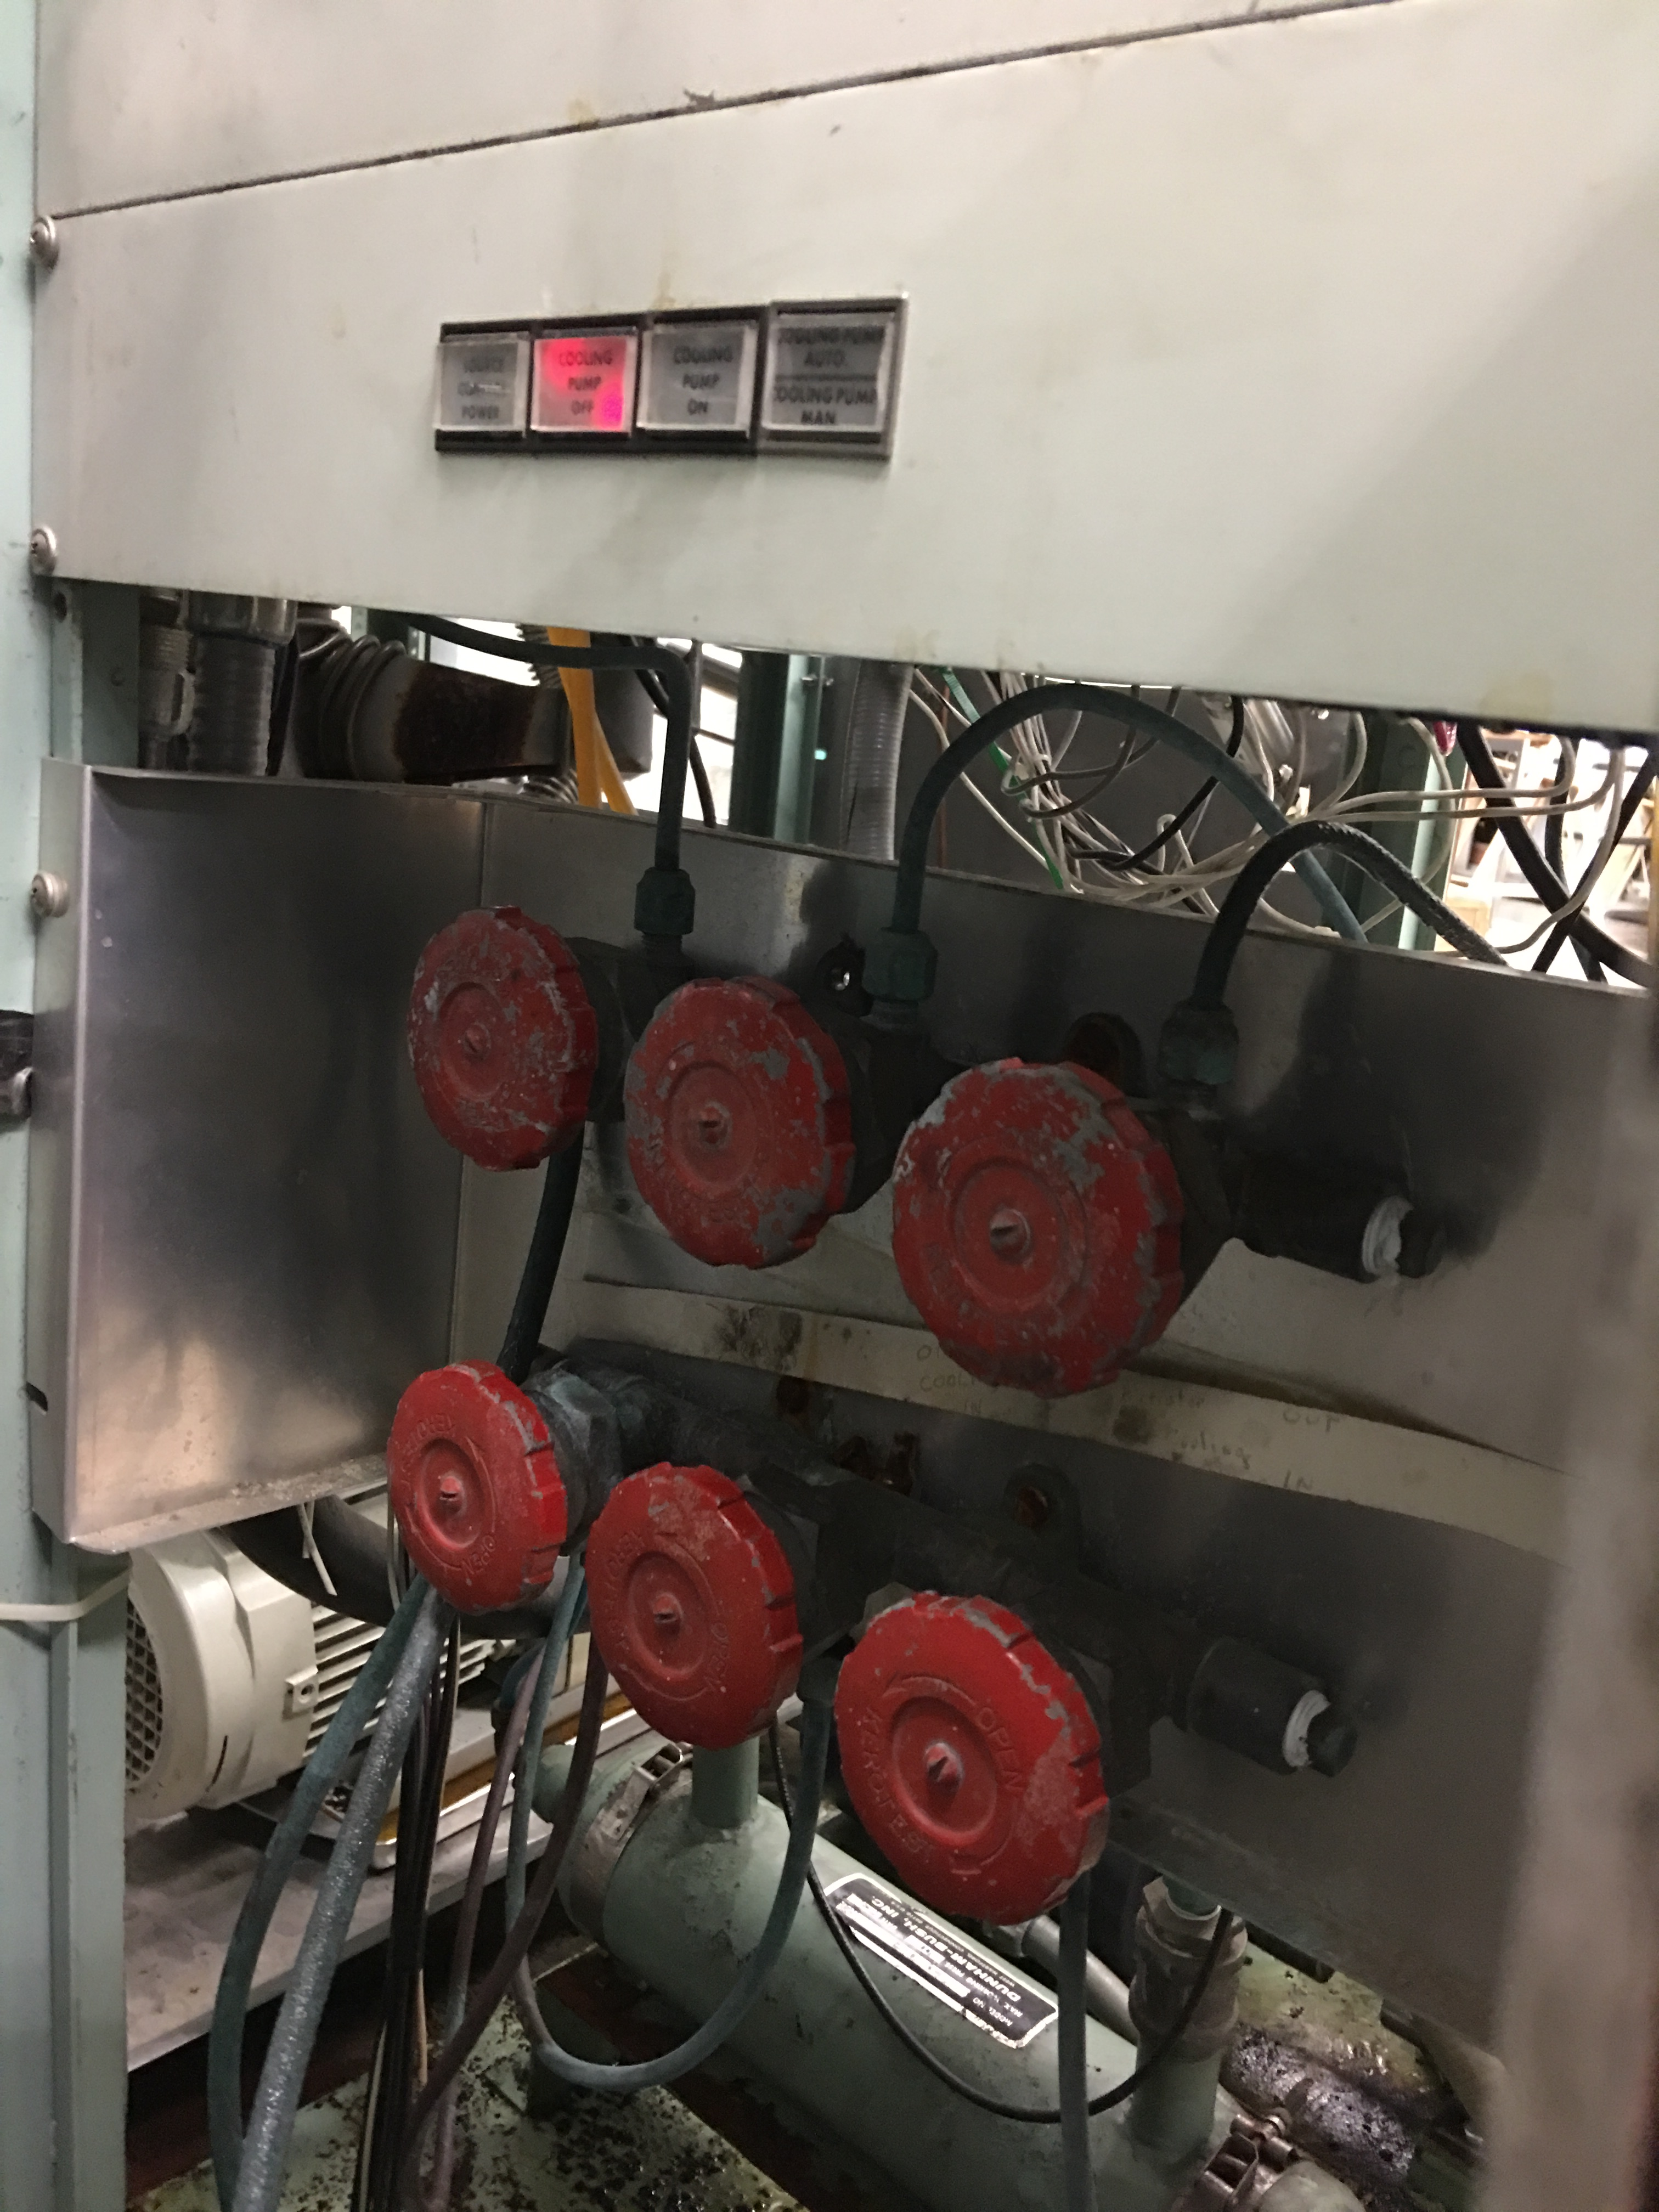
\includegraphics[width=0.5\textwidth]{IMG_0384}\\
\end{center}
\caption{\label{figure9}Water valves for cooling water. They are found behind the panel where the $^{4}$He source manifold is located in the low energy bay.}
\end{figure}

\begin{figure}
\begin{center}
\includegraphics[width=0.5\textwidth]{IMG_0385}\\
\end{center}
\caption{\label{figure10}Freon pump switch, Freon tube and flow meter with its paddle wheel on the top. These are found in the low energy bay on the side of the helium source control panel.}
\end{figure}

\begin{figure}
\begin{center}
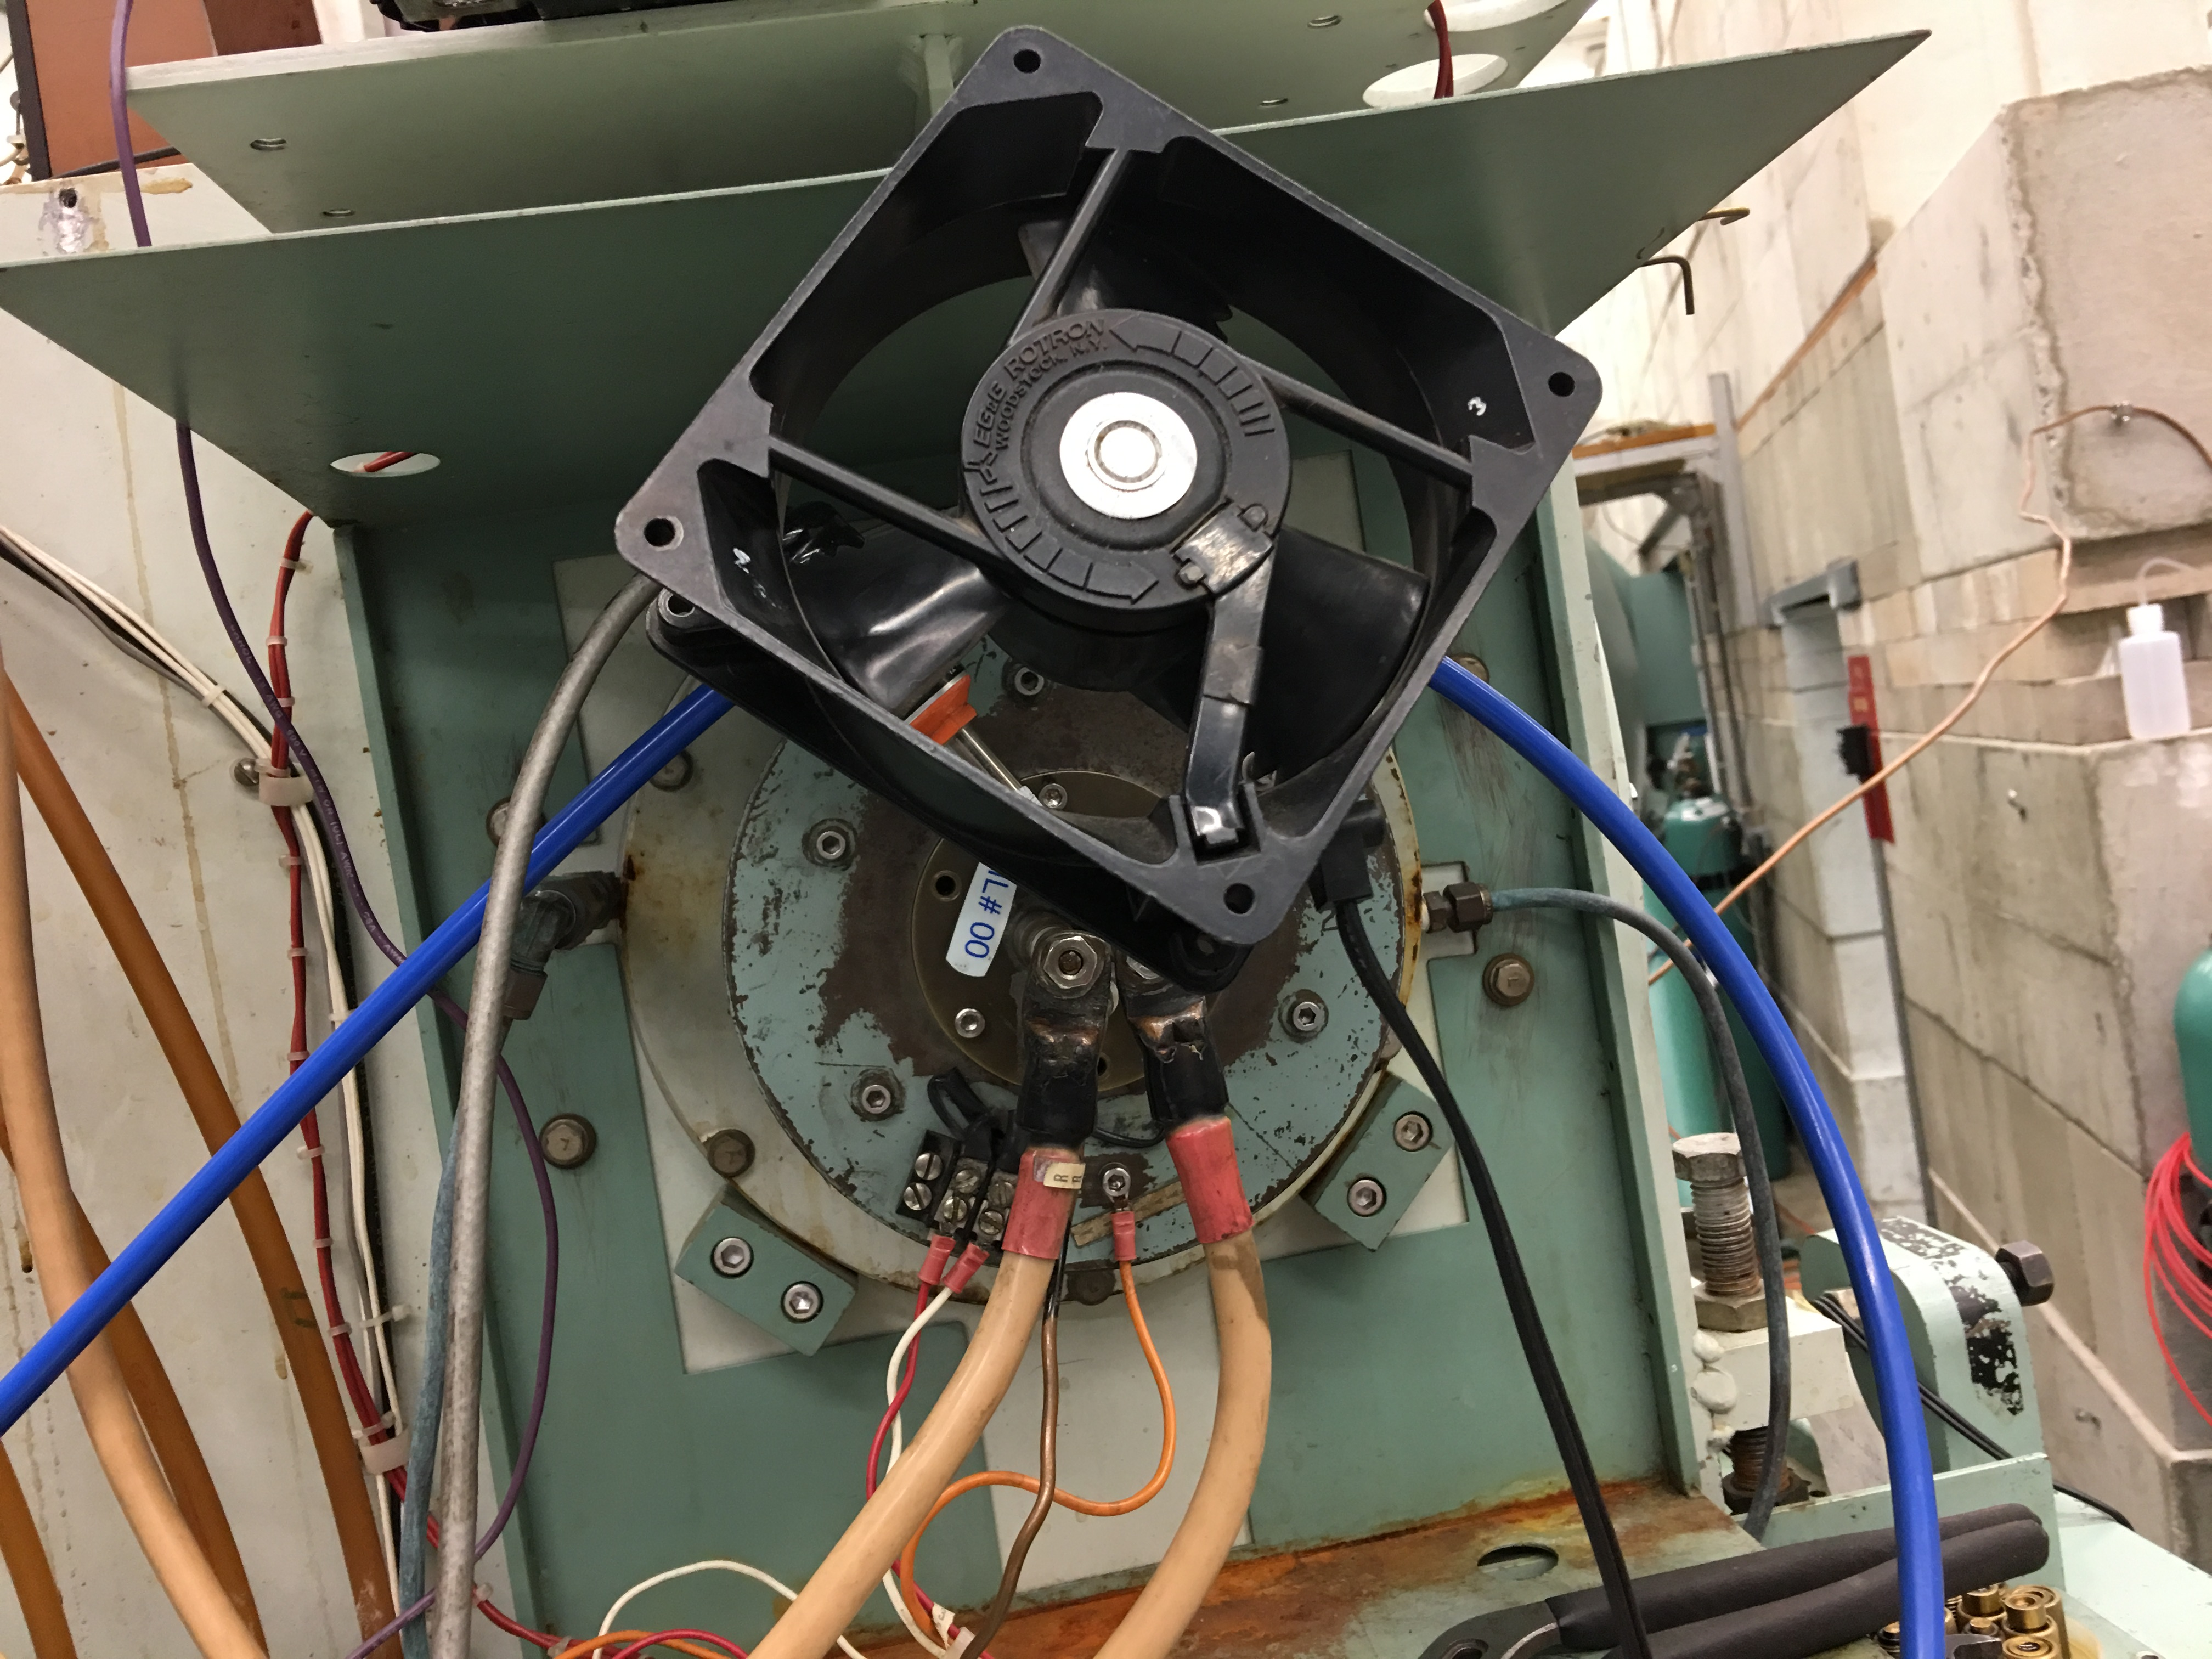
\includegraphics[width=0.5\textwidth]{IMG_0386}\\
\end{center}
\caption{\label{figure11}Filament Fan whose power cable has a big yellow plug. This fan is on the top of the helium source control panel.}
\end{figure}

\begin{figure}
\begin{center}
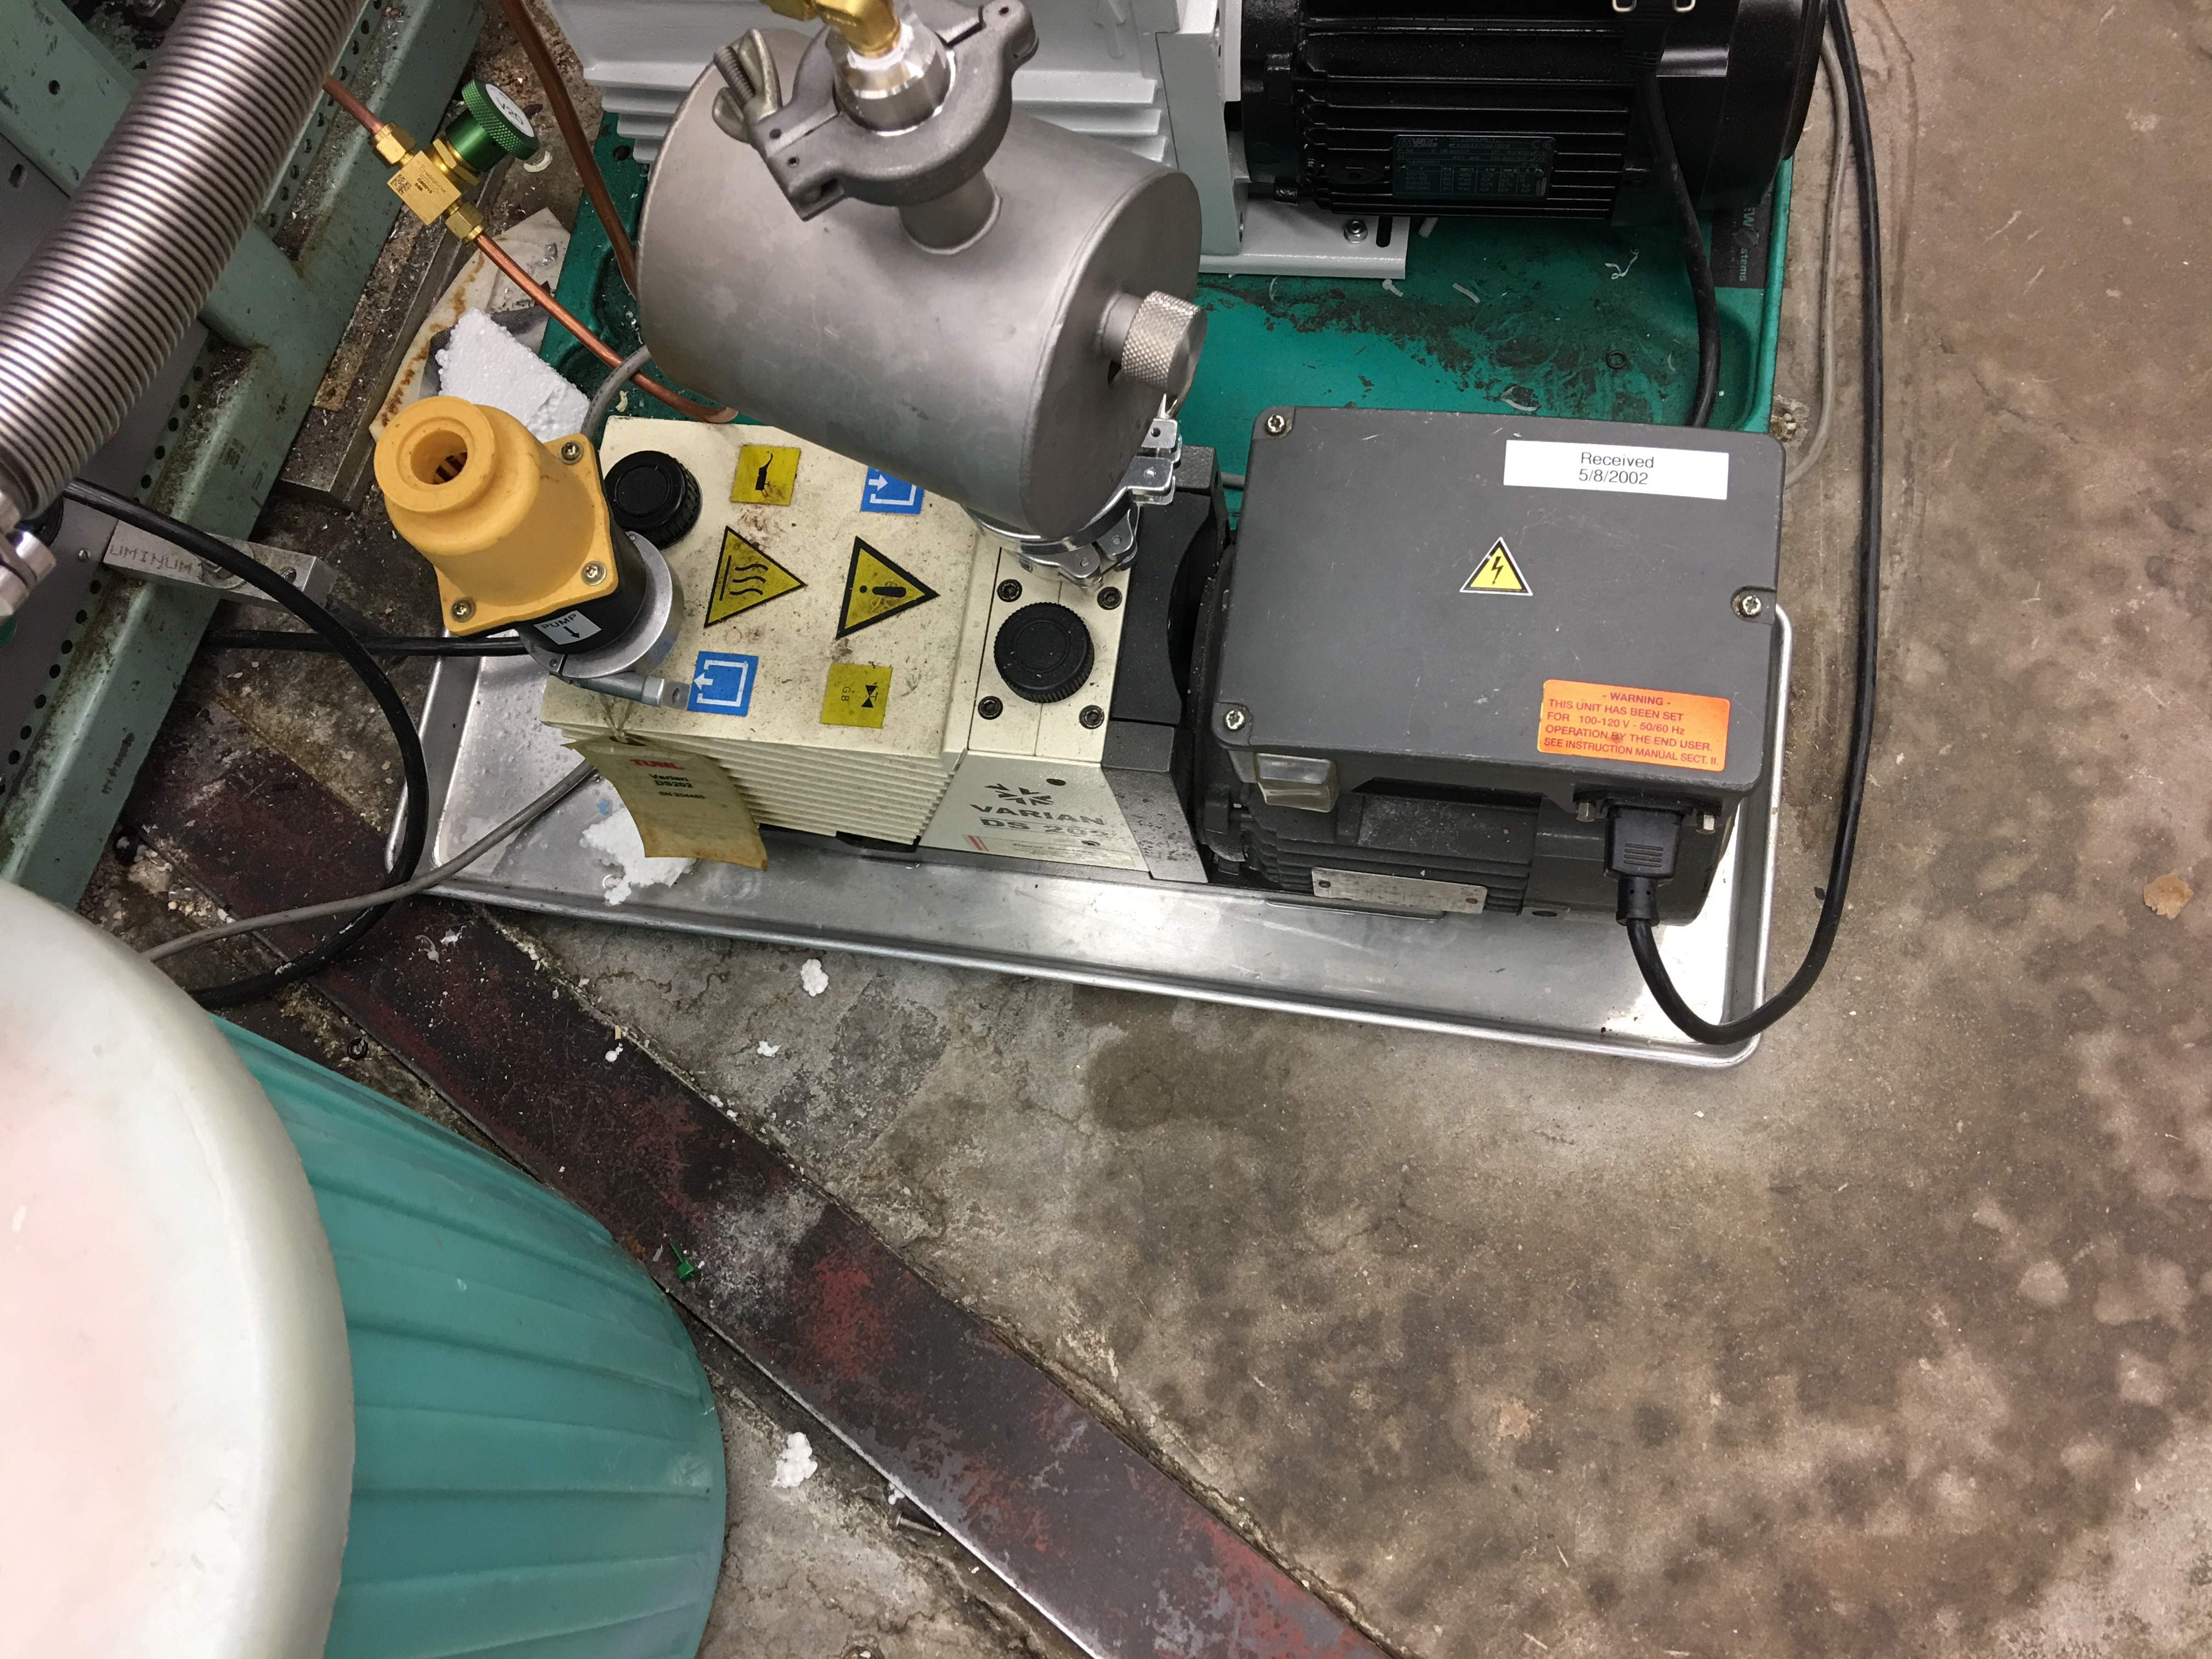
\includegraphics[width=0.5\textwidth]{IMG_0388}\\
\end{center}
\caption{\label{figure12}$^{4}$He roughing pump found underneath the wooden box beside the helium source.}
\end{figure}

\begin{figure}
\begin{center}
\includegraphics[width=0.5\textwidth]{IMG_0389}\\
\end{center}
\caption{\label{figure13}A mechanical gauge which reads the pressure within the top manifold.}
\end{figure}

\begin{figure}
\begin{center}
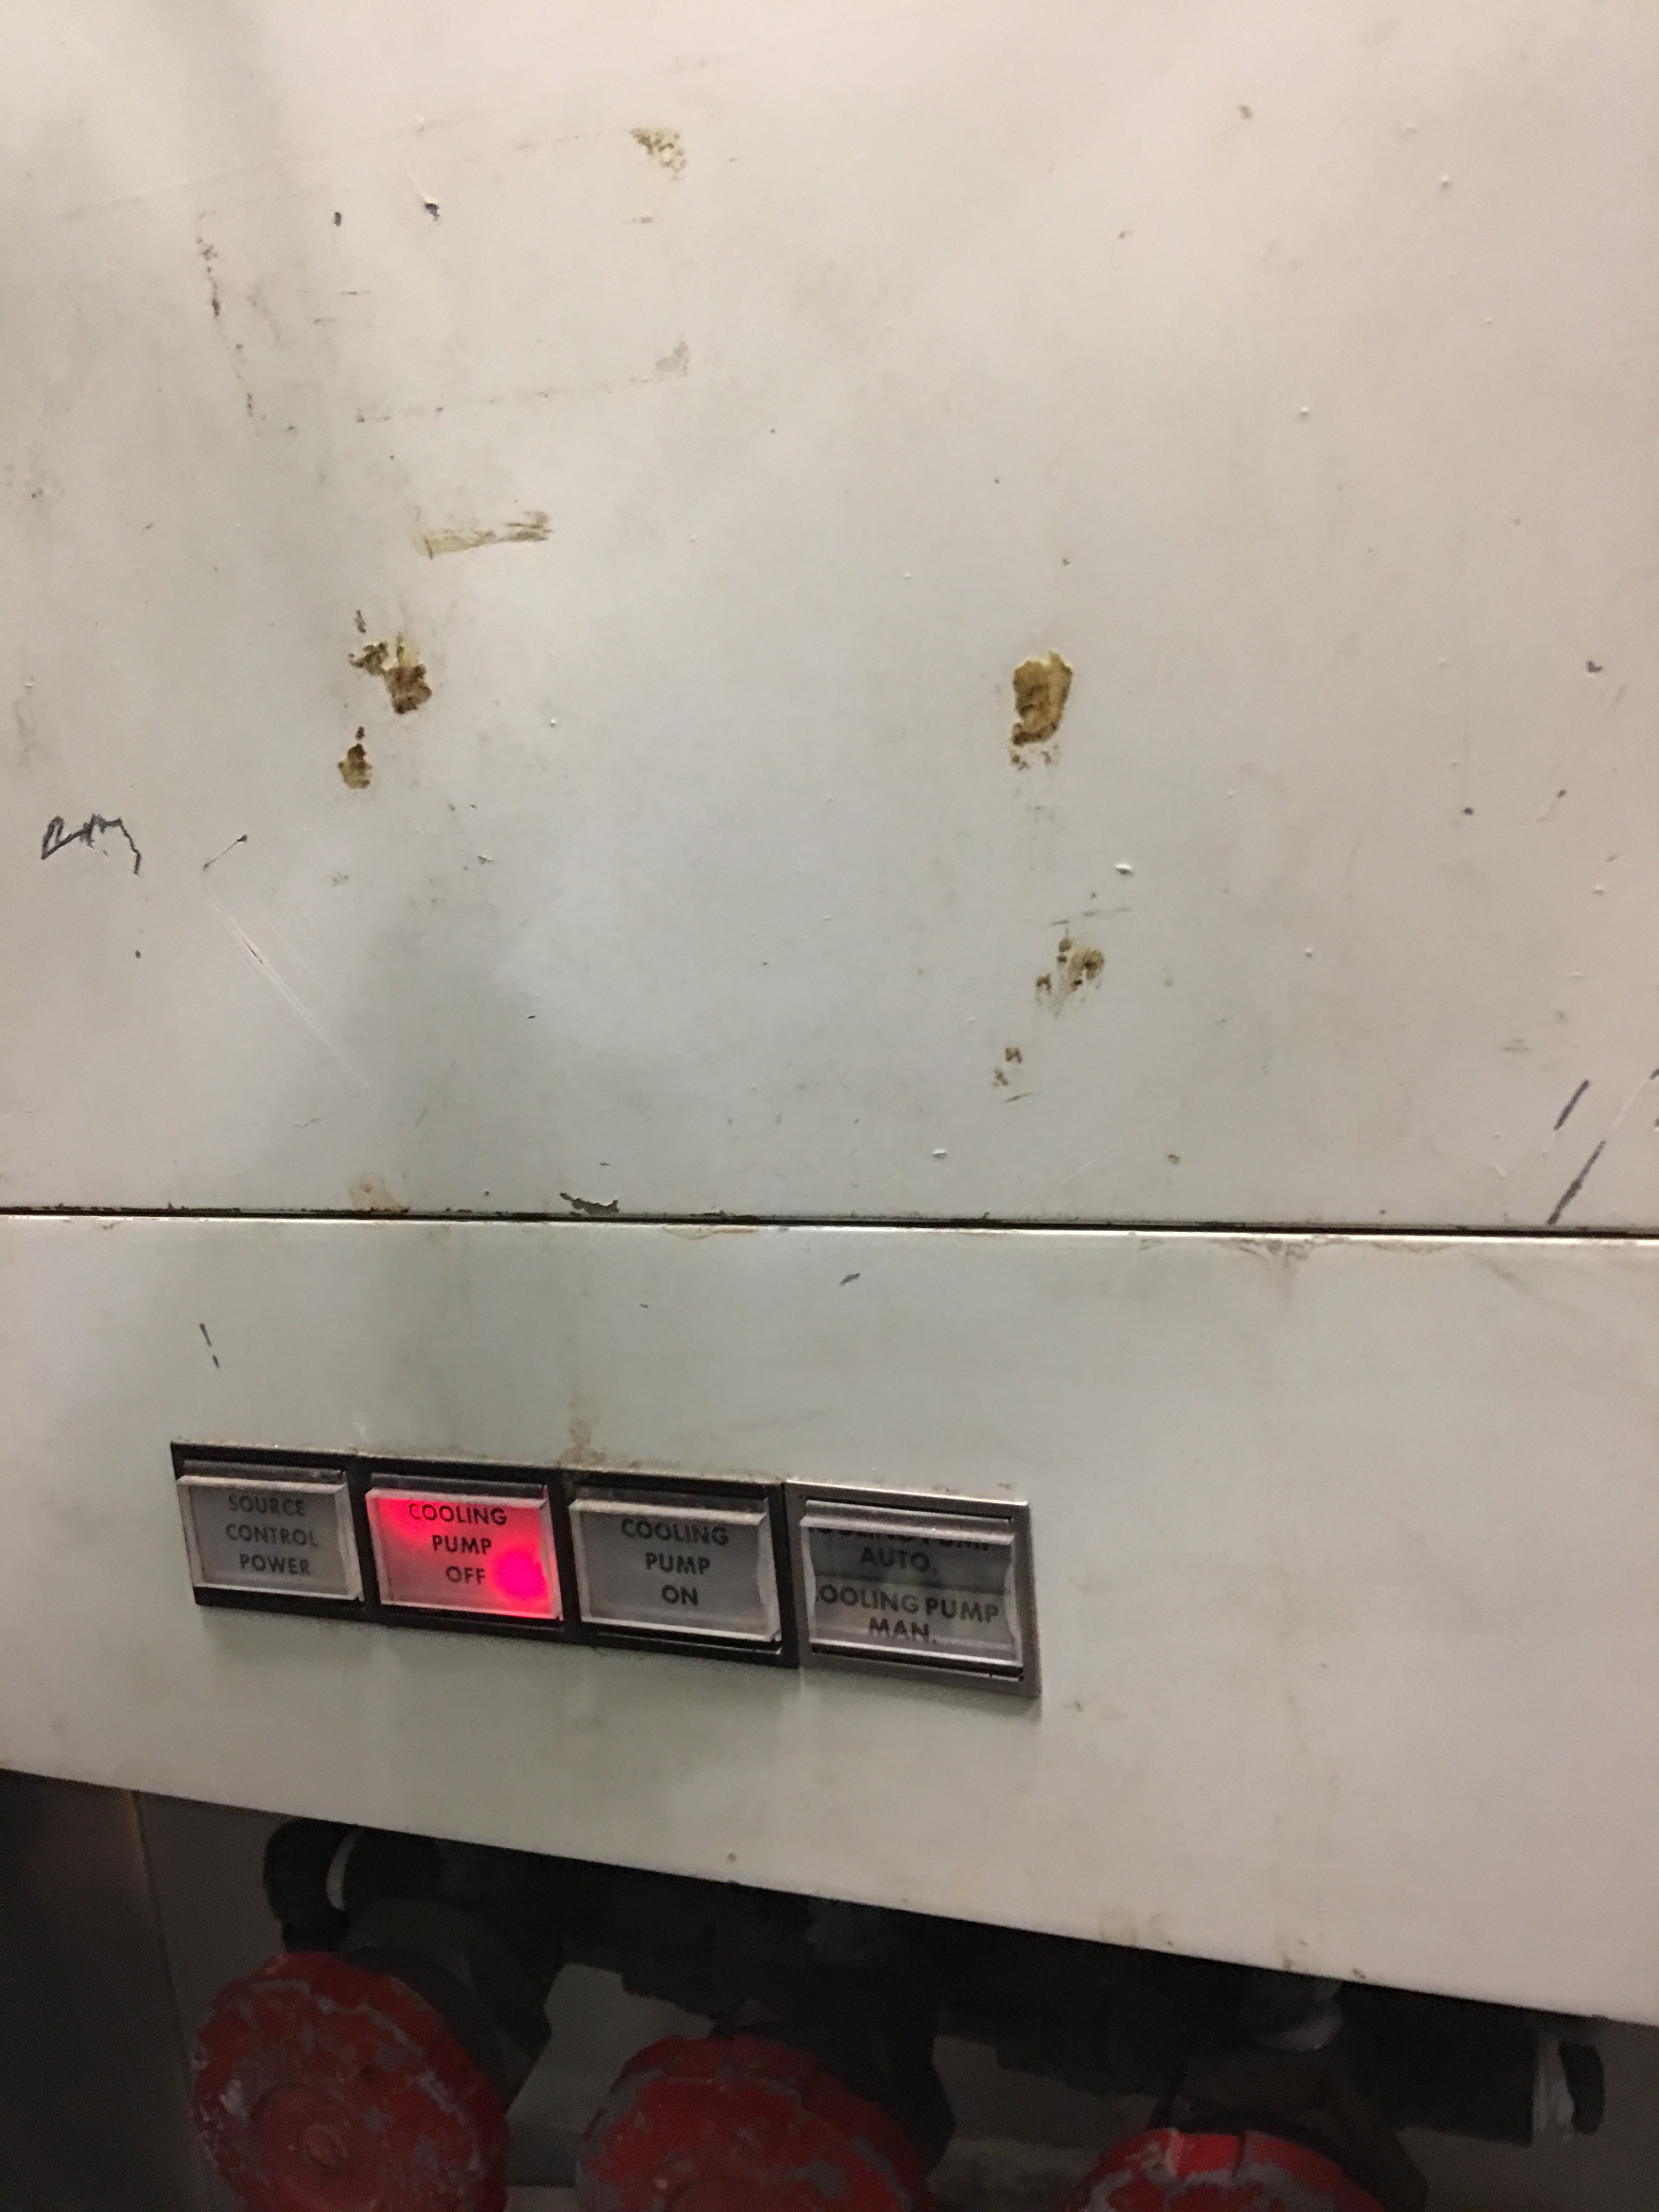
\includegraphics[width=0.5\textwidth]{IMG_0391}\\
\end{center}
\caption{\label{figure14}Switch for cooling oil pump. It is found in the low energy bay behind the alpha source panel.}
\end{figure}

\begin{figure}
\begin{center}
\includegraphics[width=0.5\textwidth]{IMG_0401}\\
\end{center}
\caption{\label{figure15}Cooling oil pressure Gauge (the bottom gauge) in the low energy bay at the helium source. The top gauge shows foreline pressure for $^{3}$He recovery system. This pressure should be low and if it is not, try to unplug the associated thermocouple found close to the alpha source diffusion pump and plug it back in until the gauge reads correctly.}
\end{figure}

\begin{figure}
\begin{center}
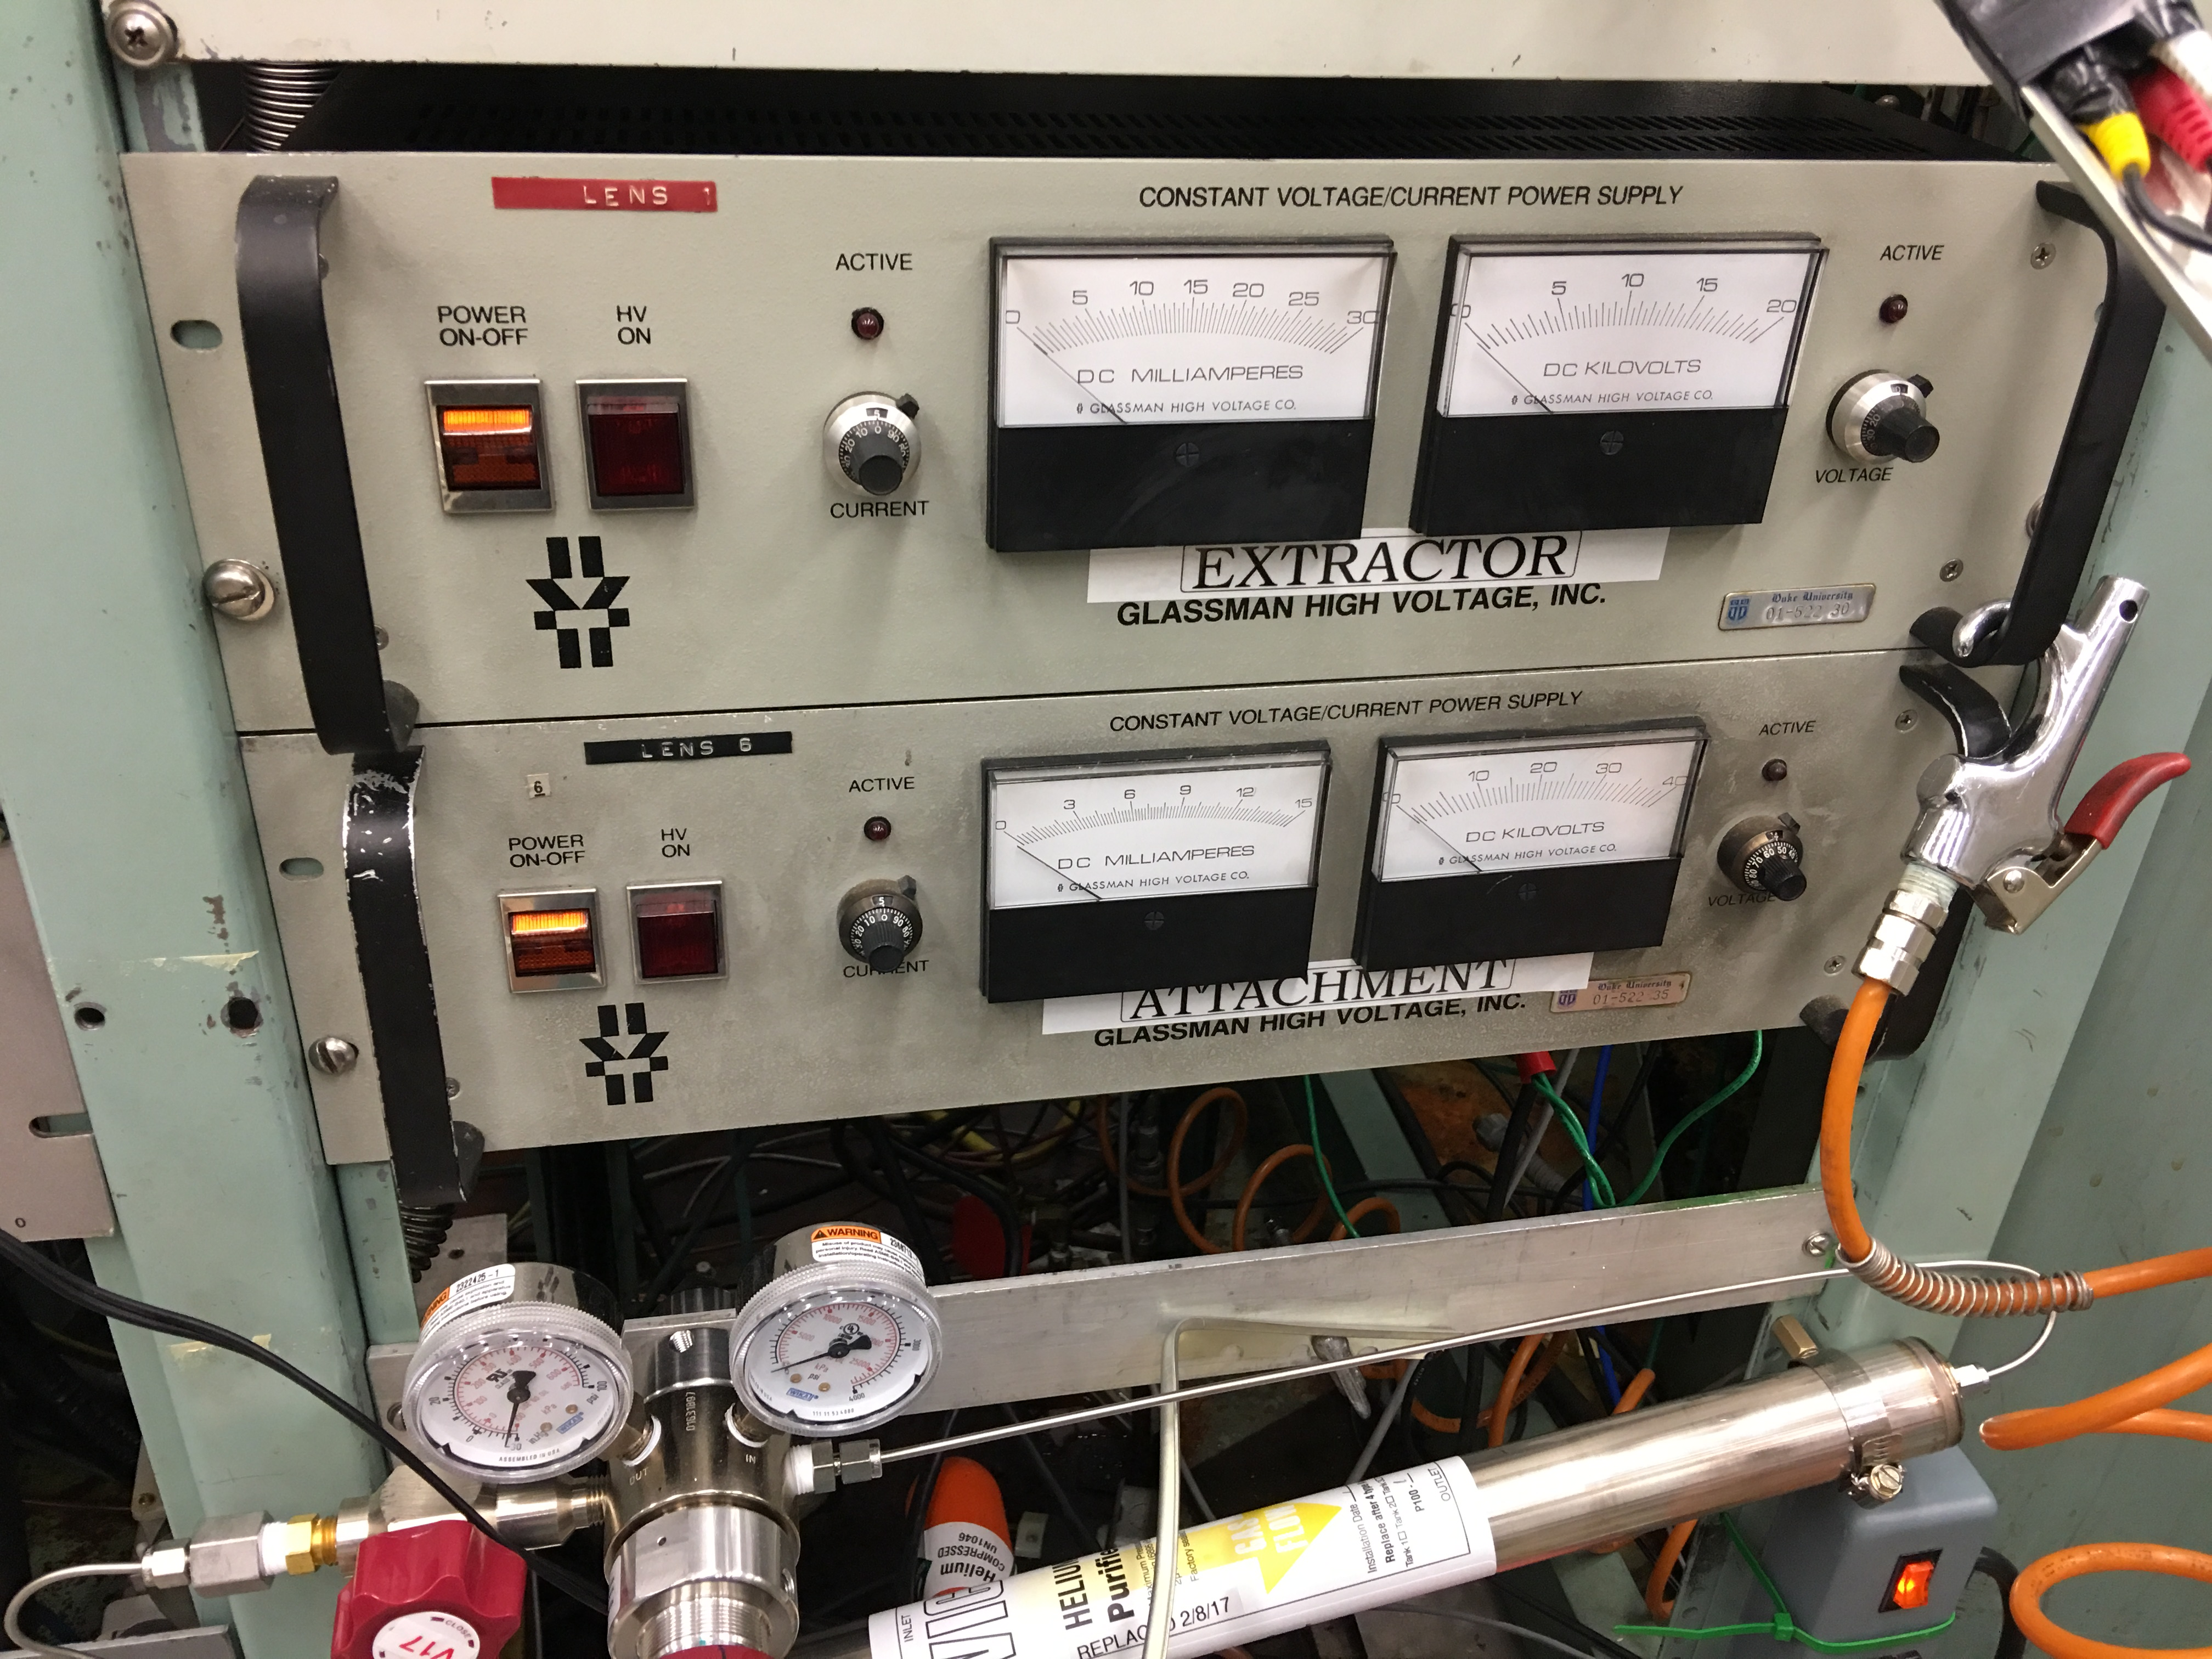
\includegraphics[width=0.5\textwidth]{IMG_0393}\\
\end{center}
\caption{\label{figure16}The attachment and extractor electrodes power supplies. They are found in the low energy bay at the helium source panel.}
\end{figure}

\begin{figure}
\begin{center}
  \subfigure[Main patch panel to the right of the low energy bay entrance door opposite of the elevator.]{%
    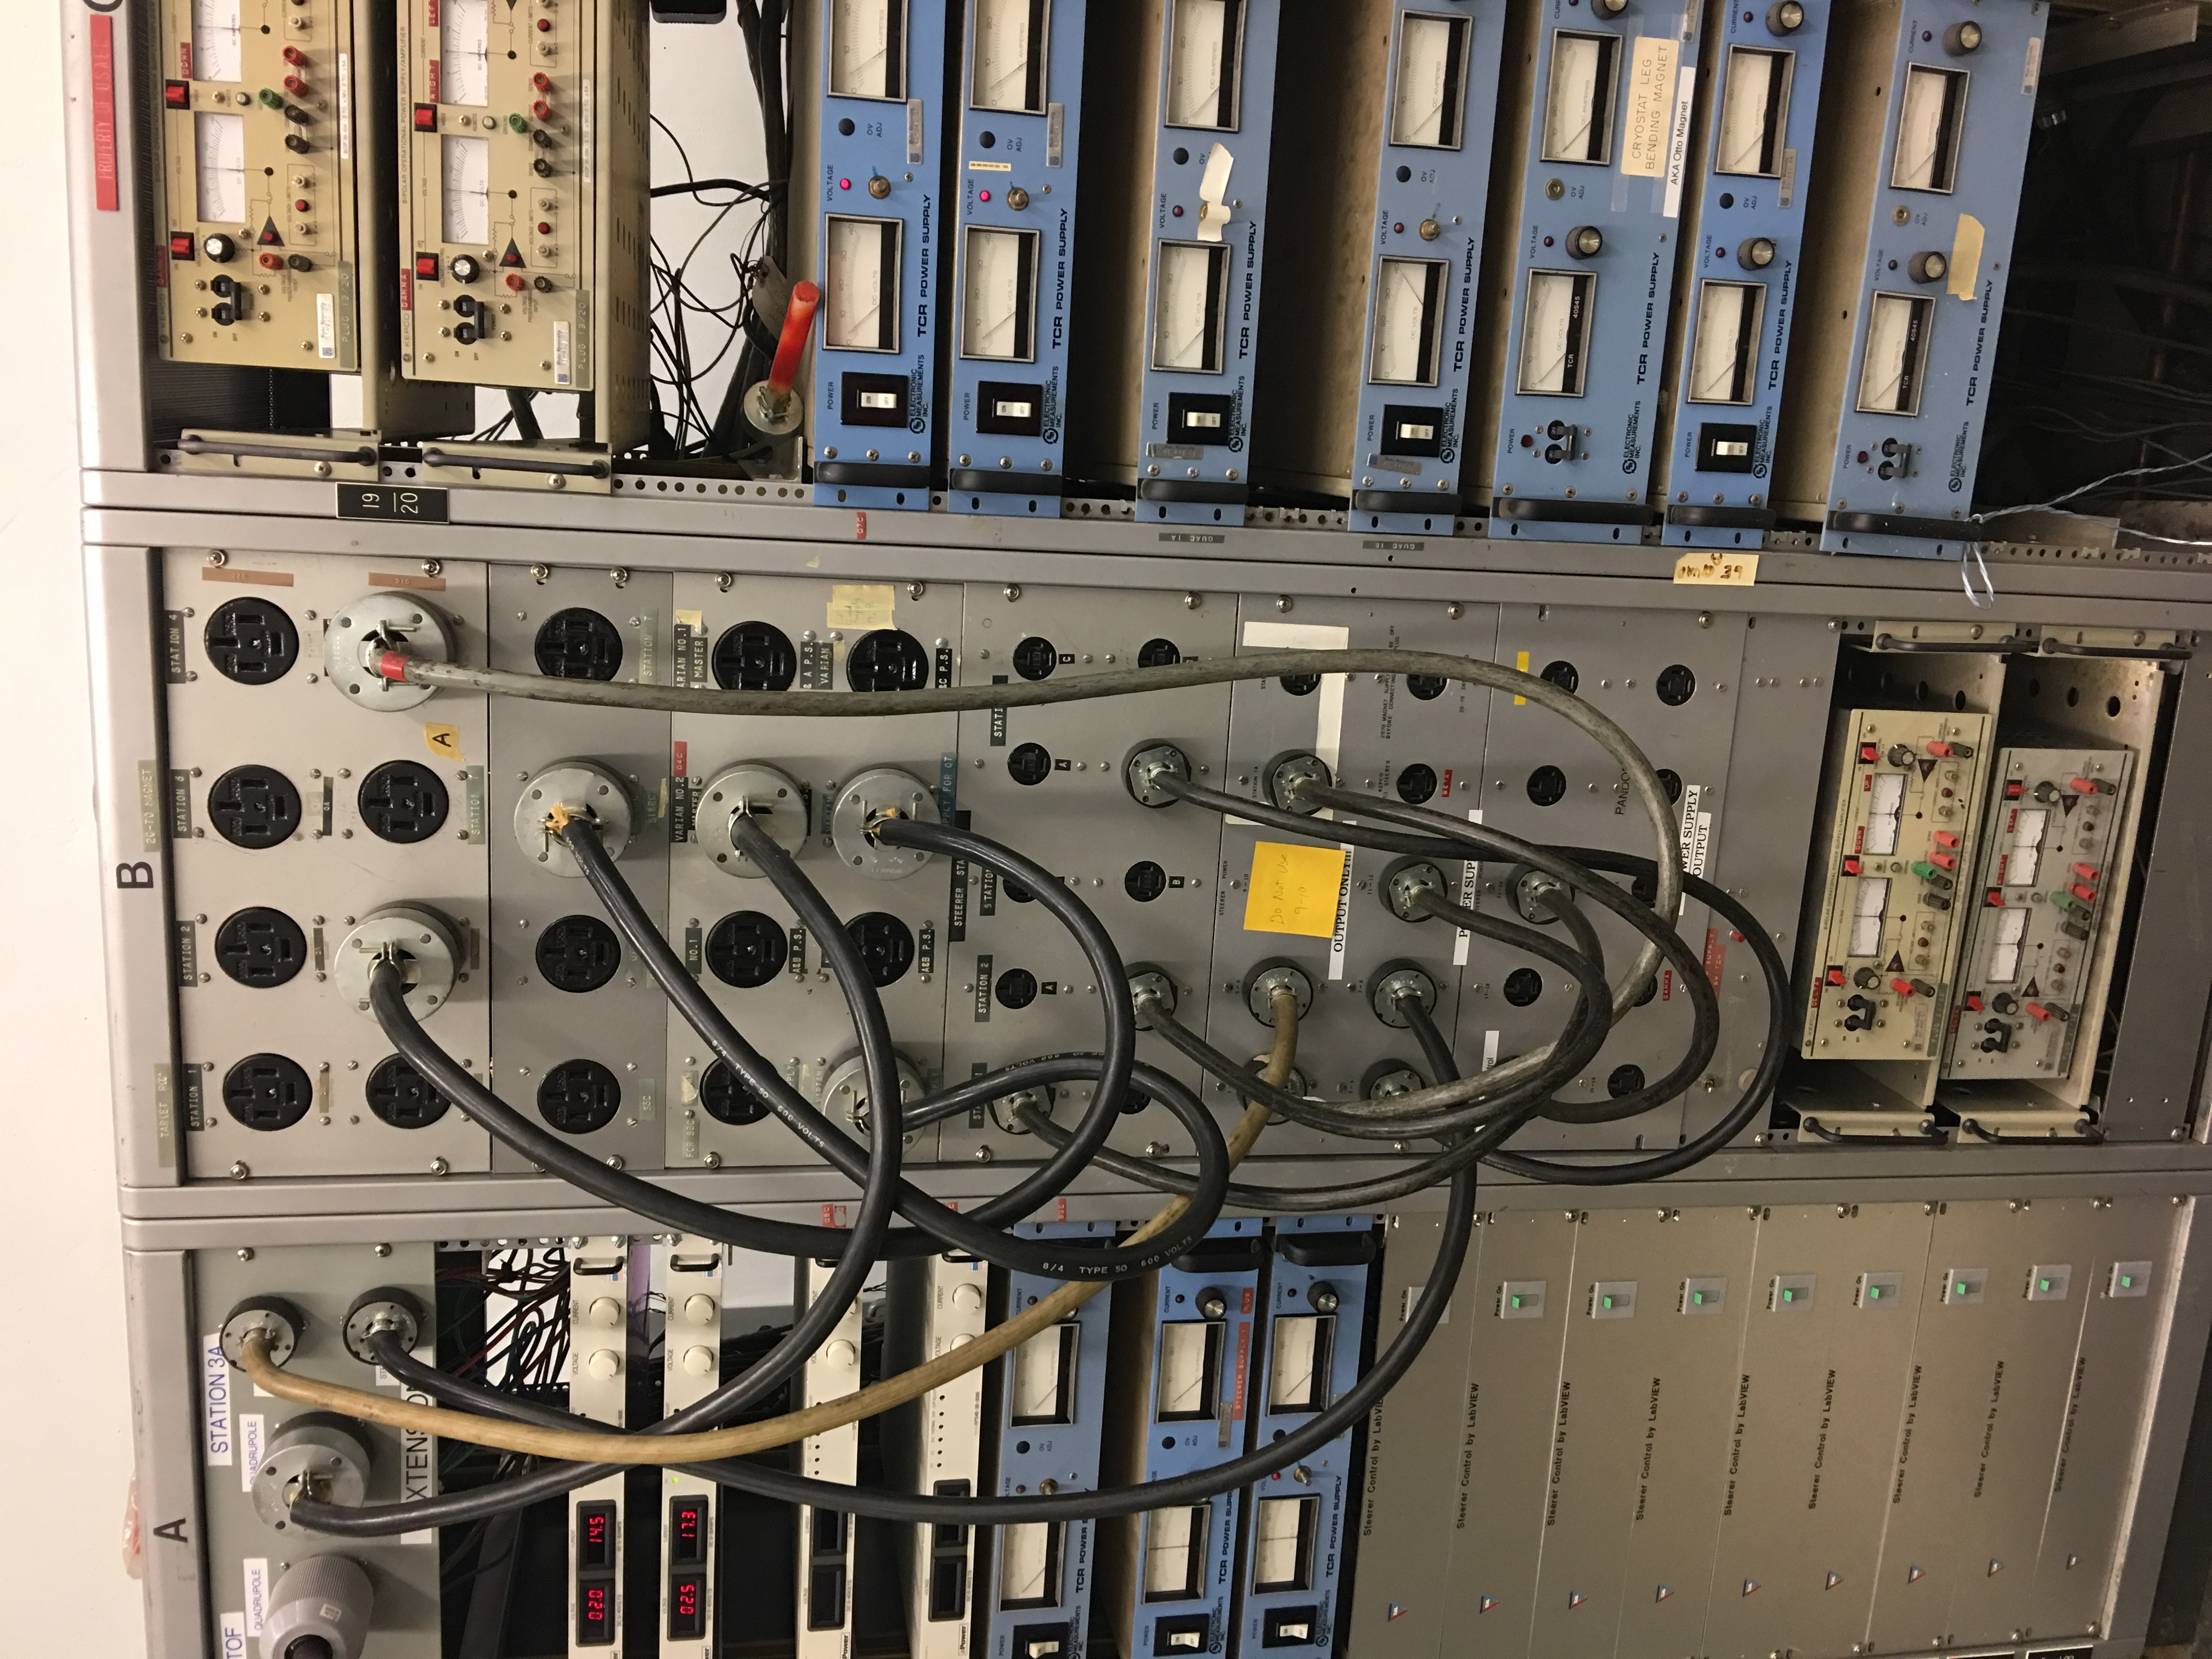
\includegraphics[width=.4\textwidth]{IMG_0447} \label{figure17a}
  }
  \quad
  \subfigure[Patch panel behind the helium source.]{%
    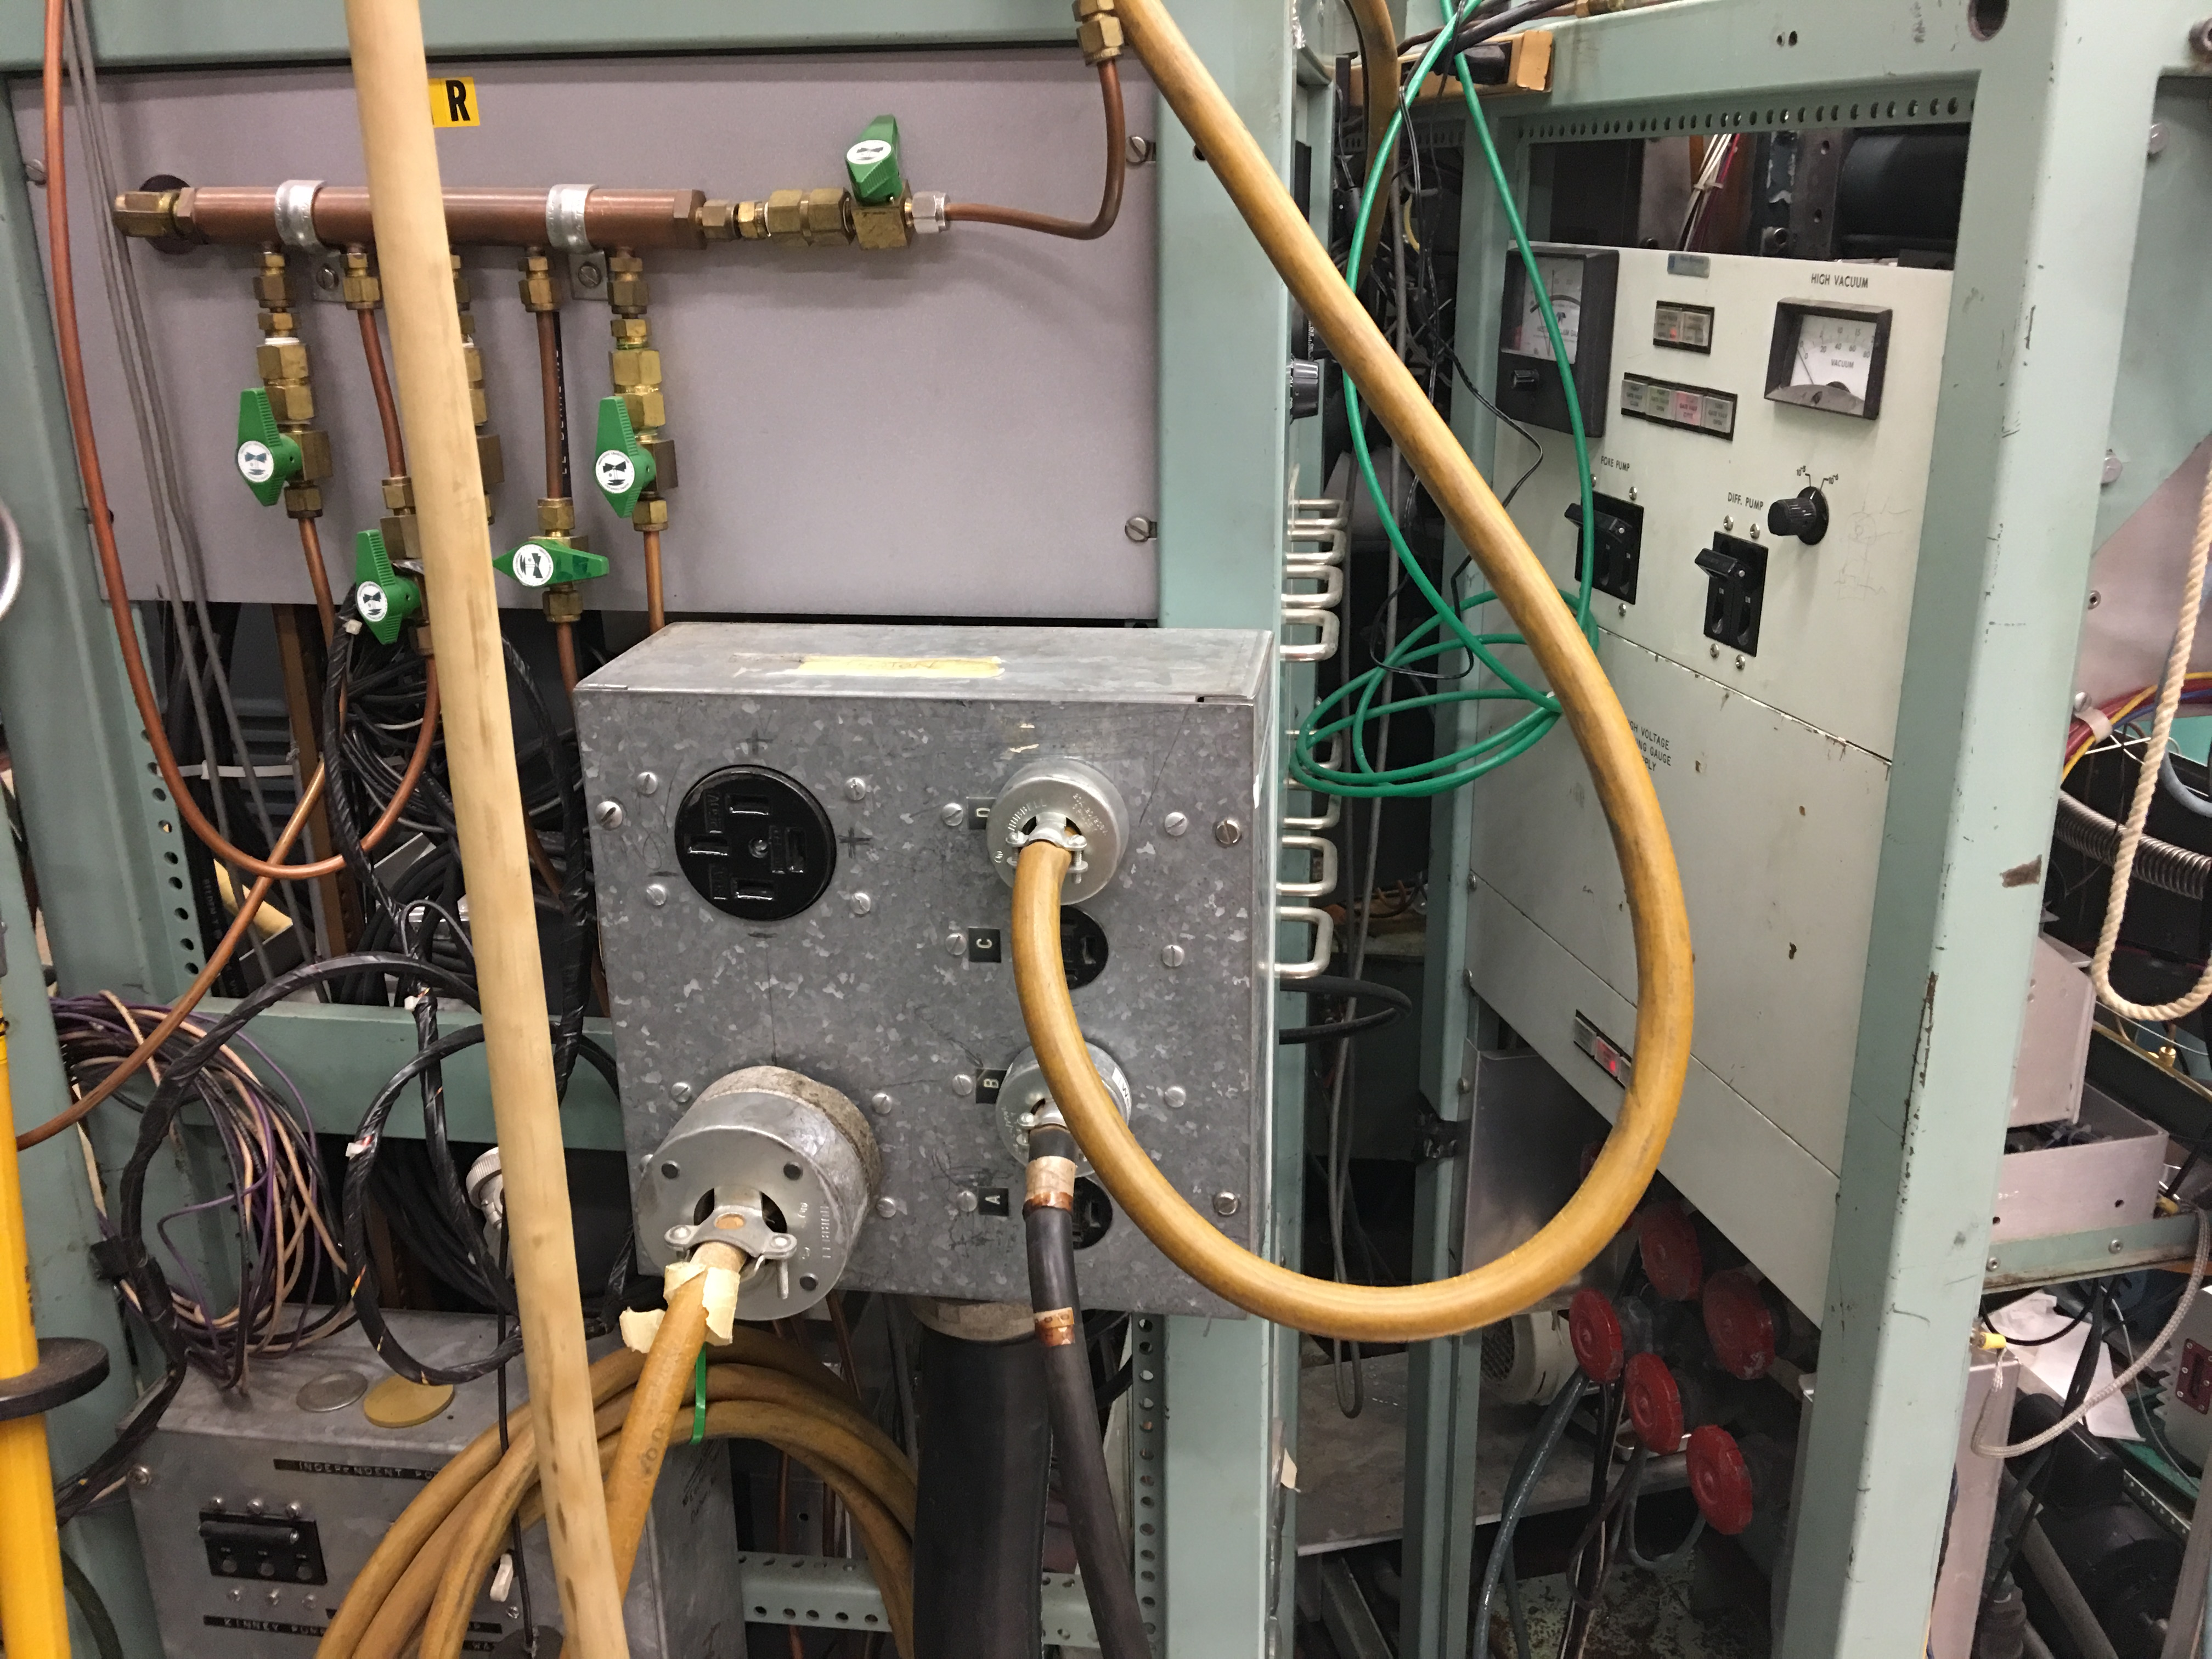
\includegraphics[width=.4\textwidth]{IMG_0446} \label{figure17b}
  }
\end{center}
  \caption{\label{figure17}hese patch panels are where the Wender steerer as well as the helium source steerer, among other things, are patched.}
\end{figure}

\section{Switching to $^{3}$He}
\label{he-3_beam}

$\bullet$ Fig.~\ref{figure20} shows the schematics of the $^{3}$He recovery system with all the valves and their connecting pipes. Please refer to this figure while following the instructions below.\\
$\bullet$ Go to low energy bay where the $^{3}$He recovery system is.\\
$\bullet$ Make sure these valves are closed: V11, V7, V14 and V12.\\
$\bullet$ Turn on compressor and $^{3}$He rotary vane pump (see Fig.~\ref{figure21}).\\
$\bullet$ Open valve V9.\\
$\bullet$ Turn on the $^{4}$He roughing pump (see Fig.~\ref{figure12}).\\
$\bullet$ Open valves V20, valve to $^{3}$He recovery, V10, V13 and V17.\\
$\bullet$ Wait for 30 minutes of pumping, and fill liquid nitrogen dewar during this waiting time. The liquid nitrogen may boil quickly the first time you fill it, so please check the level and make sure the dewar is filled to the top.\\
$\bullet$ The foreline pressure gauge seen on the top of Fig.~\ref{figure15} should be somewhere below 50 mTorr. If not, try to unplug the associated thermocouple gauge and plug it back in. This should fix the gauge and it should read less than 50 mTorr.\\
$\bullet$ After 30 minutes, close V10, valve to $^{3}$He recovery and V20.\\
$\bullet$ Turn the $^{4}$He roughing pump off.\\
$\bullet$ Get the key for $^{3}$He gas bottle from the key storage in the control room.\\
$\bullet$ Open the lock on $^{3}$He gas bottle. Decrease regulator R2 all the way out. Open $^{3}$He bottle for 2 seconds. Then close it. Open valve V12. Very very slowly increase regulator R2 until G1 pressure gauge reads 0.05 psi. Close valve V12. Continue this process until G1 pressure gauge reads 0.5 psi.\\
$\bullet$ Make sure $^{3}$He gas bottle and valve V12 are closed and the R2 regulator is decreased all the way out. Put the lock back on the $^{3}$He bottle and return the key to the safe.\\
$\bullet$ Next, we need to pump on the $^{4}$He manifold.\\
$\bullet$ Close both valves on the $^{4}$He gas bottle.\\
$\bullet$ Close valve V1.\\
$\bullet$ Turn on the $^{4}$He roughing pump.\\
$\bullet$ Open valves V20, valve to helium source manifold and V18.\\
$\bullet$ Once the flow meter seen in Fig.~\ref{figure2} reads zero sccm, close valves V18, V19, valve to helium source manifold, and V20.\\
$\bullet$ Turn off the $^{4}$He roughing pump.\\
$\bullet$ Make sure valves V13 and V17 are open.\\
$\bullet$ Open valve V3.\\
$\bullet$ Close valve V6 and open valve V8 (both are found behind the $^{3}$He recycling panel close to the diffusion pump) to switch the backing pump for the diffusion pump. If during closing V6 and opening V8 valves, you hear a clicking sound around the diffusion pump, quickly check the foreline pressure of the diffusion pump (the gauge is at the back of the helium source pannel, see Fig.~\ref{figure8}) to see if pressure is higher than the red indicator on the gauge. If this is the case, the interlock has turned the pump and everything else off and the clicking sound is due to that. In this case, you need to quickly unplug the thermocouple gauge (which can be found behind valve V8 on the same beam pipe (NOT the thermocouple gauge on the left of valve V8)) and plug it back again and quickly make sure that the foreline pressure goes below the red indicator on the gauge. This thermocouple gauge seems to be loose and if you wiggle things around it, it may disconnect a wire there which will engage with the interlock and turn the diffusion pump off.\\
$\bullet$ Go to control room.\\
$\bullet$ Raise the gas source needle valve until the flow meter seen in Fig.~\ref{figure2} reads 0.5 sccm. At this point, the helium source filament pressure gauge should be 0.2 Torr. If not, gently raise or lower the gas source needle valve until the aforementioned pressure is 0.2 Torr.\\
$\bullet$ Change the NIS magnet to $\sim$66 mA and tune $^{3}$He beam on the low energy cup.

\begin{figure}
\begin{center}
\includegraphics[width=0.5\textwidth]{IMG_0381}\\
\end{center}
\caption{\label{figure18}Sodium oven switch and knob for changing sodium oven heater current. Both can be found in the control room.}
\end{figure}

\begin{figure}
\begin{center}
\includegraphics[width=0.5\textwidth]{IMG_0396}\\
\end{center}
\caption{\label{figure19}The air cooling valve to cool the sodium oven with air. This valve is found in the low energy bay at the helium source panel on the top left side.}
\end{figure}

\begin{figure}
\begin{center}
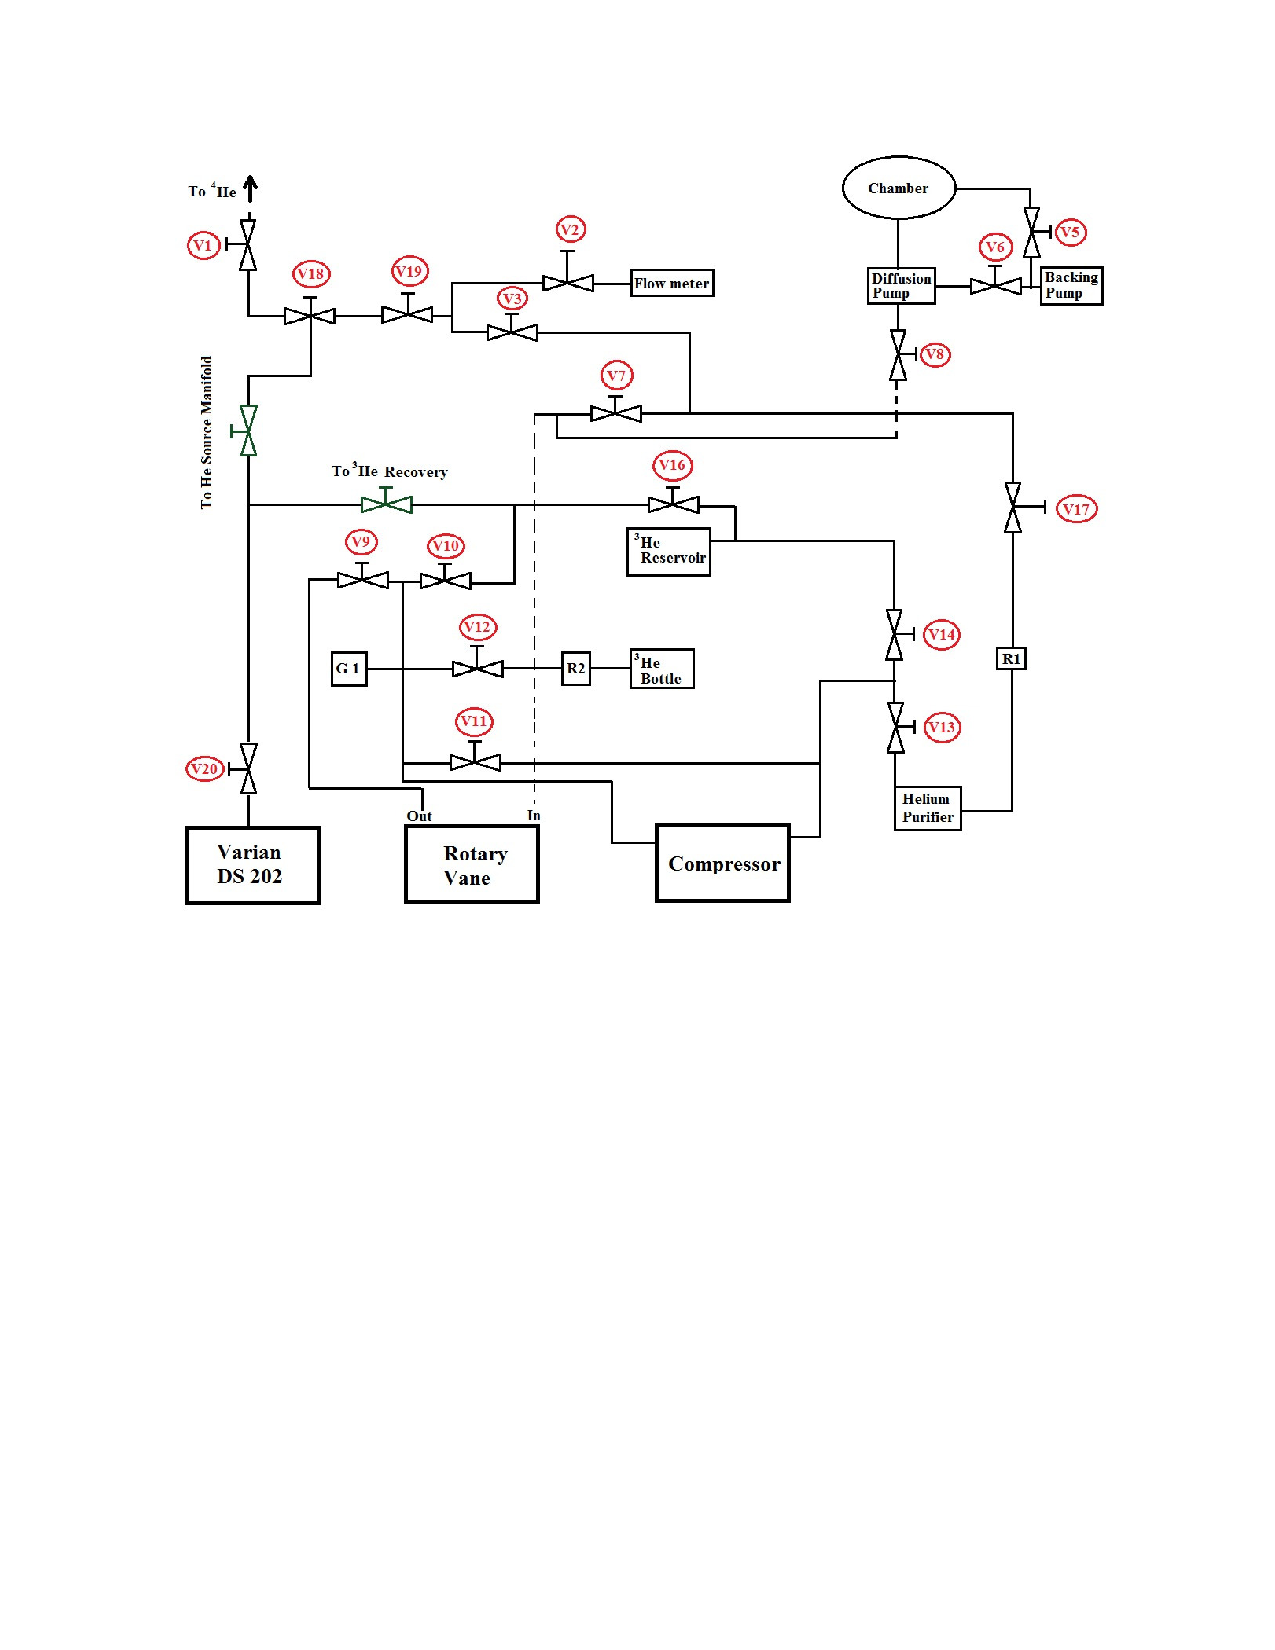
\includegraphics[width=\textwidth]{He_Source_Valve_Diagram}\\
\vspace{-10cm}
\end{center}
\caption{\label{figure20}Schematics of the $^{3}$He recovery system.}
\end{figure}

\begin{figure}
\begin{center}
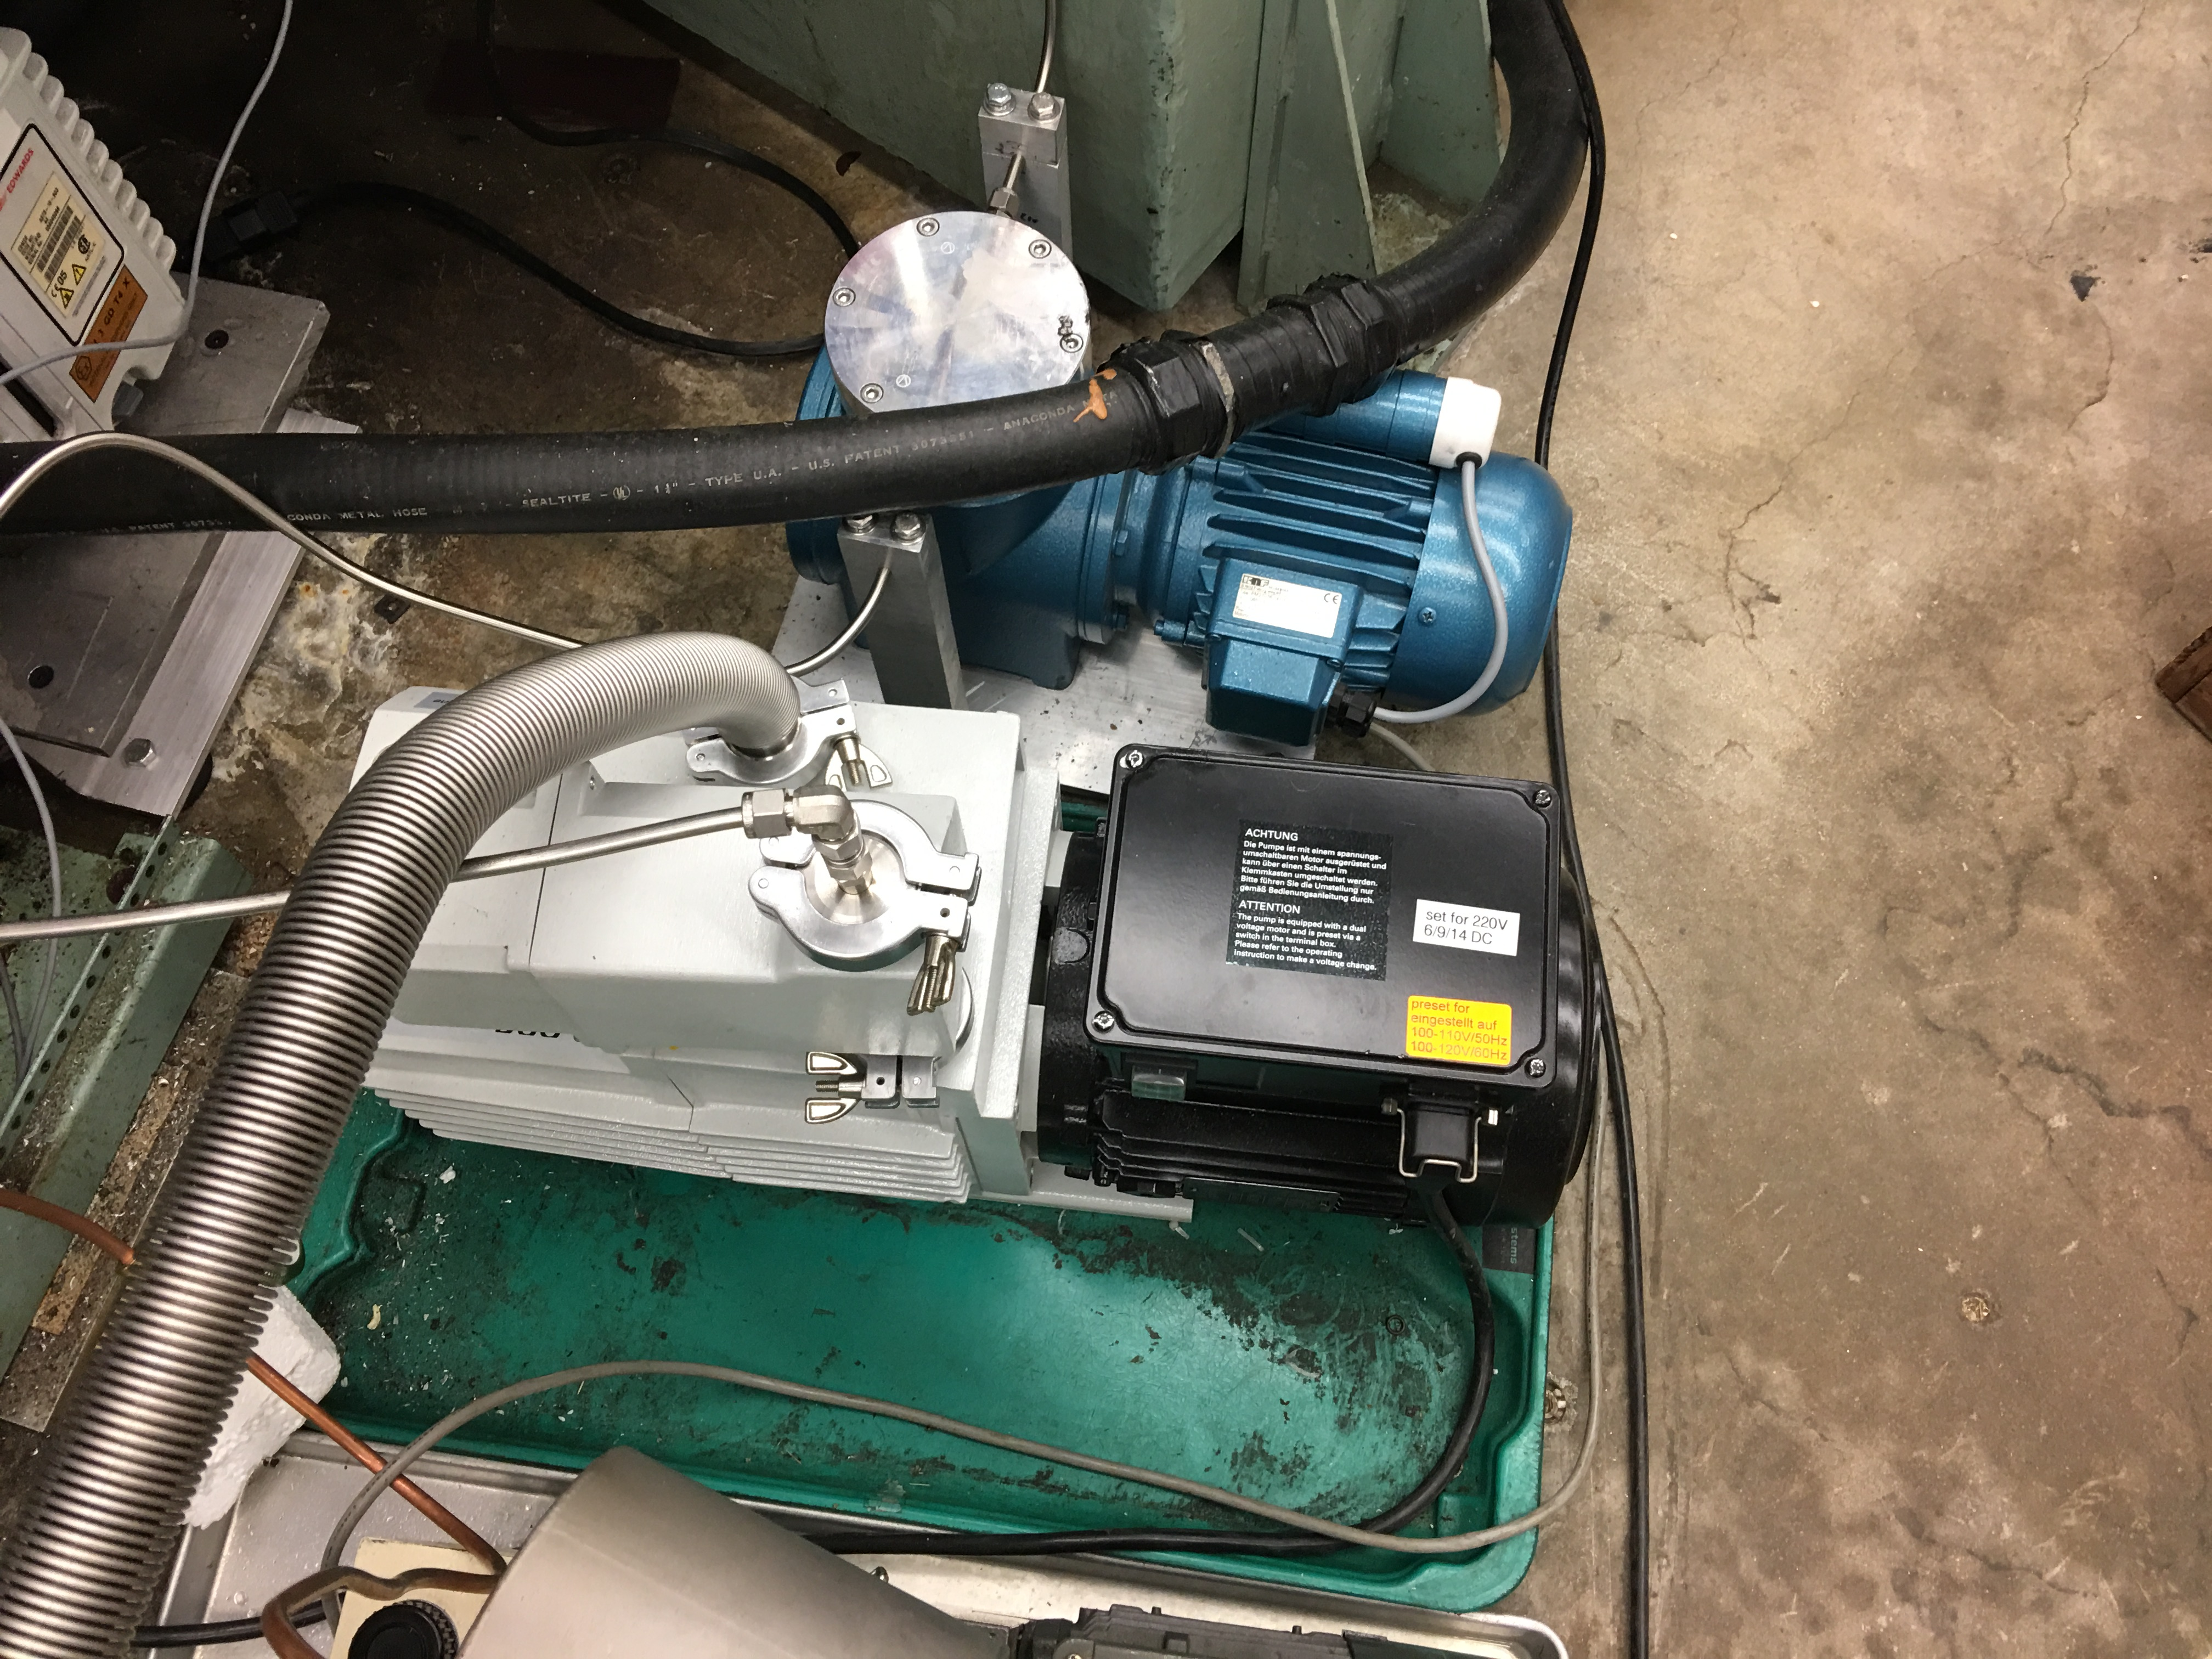
\includegraphics[width=0.5\textwidth]{IMG_0394}\\
\end{center}
\caption{\label{figure21}The rotary vane pump and compressor used to recycle $^{3}$He gas.}
\end{figure}

\section{Putting the Ion Source to Sleep Mode}

With beam fully on (the arc current should be non-zero) and without touching anything on the ion source:\\
$\bullet$ Turn down the sodium oven heater current knob in the control room until the oven heater current goes to zero, and then switch the sodium oven off.\\
$\bullet$ DO NOT turn off tandem control power switch and DO NOT turn off helium source control power switch.\\
$\bullet$ Go to low energy bay.\\
$\bullet$ Open air cooling valve all the way, and wait for 30 minutes for the oven to cool down. DO NOT take the beam away (do not lose the plasma, in other words, DO NOT touch the filament current and other source variables) at this time; otherwise, the sodium will clog the oven and next time, you will not get any beam.\\
$\bullet$ Log sodium oven usage hours on a sheet of paper posted on the helium source at low energy bay.\\
$\bullet$ After 30 minutes, close air cooling valve.\\
$\bullet$ Close helium source gate valve using a screw driver and turning the little screw on the valve's body counter clockwise.\\
$\bullet$ Close low energy tube gate valve.\\
$\bullet$ If you are using the $^{4}$He beam, stop here.\\
$\bullet$ If you are using $^{3}$He beam, continue:\\
$\bullet$ Close valves V3, V13 and V17 found on the $^{3}$He recycling system.\\
$\bullet$ Close valve V8 and open valve V6 to switch the backing pump for the diffusion pump. If during closing V8 and opening V6 valves, you hear a clicking sound around the diffusion pump, quickly check the foreline pressure of the diffusion pump (the gauge is at the back of the helium source pannel, see Fig.~\ref{figure8}) to see if pressure is higher than the red indicator on the gauge. If this is the case, the interlock has turned the pump and everything else off and the clicking sound is due to that. In this case, you need to quickly unplug the thermocouple gauge (which can be found behind valve V8 on the same beam pipe (NOT the thermocouple gauge on the left of valve V8)) and plug it back again and quickly make sure that the foreline pressure goes below the red indicator on the gauge. This thermocouple gauge seems to be loose and if you wiggle things around it, it may disconnect a wire there which will engage with the interlock and turn the diffusion pump off.\\
$\bullet$ Turn off $^{3}$He rotary vane pump.\\
$\bullet$ Turn off compressor.\\
$\bullet$ Go back to the control room.\\
$\bullet$ Lower source gas until the flow meter seen in Fig.~\ref{figure2} reads 0 sccm. This means the needle valve is closed and you would need to lower source gas switch for 20 seconds to do so.\\
$\bullet$ Go back to low energy bay.\\
$\bullet$ Turn on the $^{4}$He roughing pump. Open valves V20, valve to helium source manifold, V18 and V19 (valve V2 should be open already) and let the top manifold be pumped for a few minutes until the flow meter seen in Fig.~\ref{figure2} reads 0 sccm.\\
$\bullet$ Close valves V18, V19, valve to helium source manifold and V20. Turn off the $^{4}$He roughing pump.\\
$\bullet$ Open $^{4}$He gas bottle valves. Then, open valves V1 and V19.\\
$\bullet$ Go to control room, and raise the source gas switch until the flow meter seen in Fig.~\ref{figure2} reads 0.8 sccm and the helium source filament pressure is 0.2 Torr. If this pressure is not 0.2 Torr, raise or lower source gas switch until the desired filament pressure (0.2 Torr) is reached.

\section{Waking up the Ion Source}

$\bullet$ Make sure the plasma still exists (arc current is non-zero, and you can see the plasma on camera). Then:
$\bullet$ Turn on the sodium oven switch and increase oven heater current to 1 A using the big knob besides the sodium oven switch. Give it 30 minutes at 1 A and meanwhile do the following:\\
$\bullet$ Go to low energy bay.\\
$\bullet$ Open helium source gate valve using a screw driver and by turning the screw on the body of the valve clockwise.\\
$\bullet$ Open low energy tube gate valve.\\
$\bullet$ Go to control room.\\
$\bullet$ After 30 minutes, increase the oven heater current to 2.5 A and wait for 2 -- 2.5 hours for the beam intensity to go up to the desired value. Meantime, keep tunning the beam every few minutes to make sure it is maximized on the low ebergy cup.\\
$\bullet$ Once $^{4}$He beam on low energy cup is constant and steady, do the air cooling test to make sure the oven is at the right temperature.\\
$\bullet$ If you need to switch to $^{3}$He beam, do the following:\\
$\bullet$ Lower source gas until the flow meter seen in Fig.~\ref{figure2} reads 0 sccm. This means the needle valve is closed and you would need to keep pressing lower source gas switch for 20 seconds.\\
$\bullet$ Go to low energy bay where the $^{3}$He recovery system is.\\
$\bullet$ Close both valves on the $^{4}$He gas bottle.\\
$\bullet$ Close valve V1.\\
$\bullet$ Turn on the $^{4}$He roughing pump. Open valves V20, valve to helium source manifold, V18 and V19 and let the top manifold be pumped for a few minutes until the flow meter seen in Fig.~\ref{figure2} reads 0 sccm.\\
$\bullet$ Close valves V18, V19, valve to helium source manifold and V20. Turn off the $^{4}$He roughing pump.\\
$\bullet$ If the $^{3}$He source was being used the night before and the helium source was put to sleep over one night only, there must still be some good $^{3}$He in the $^{3}$He lines, and you do not need to pump that gas out. If that is the case, follow these steps; otherwise (if $^{3}$He source was not used recently and you would like to use it now), go to step $\diamond$:
\begin{itemize}
  \item Check pressure gauge G1. It should read something around 0.15 - 0.2 psi or so. It is okay if the pressure is low. Once you turn on the compressor, the pressure goes up.
  \item Fill the liquid nitrogen dwar of the recycling system.
  \item Turn on the compressor.
  \item Turn on $^{3}$He rotary vane pump.
  \item Open valves V13 and V17.
  \item If G1 pressure gauge is still lower than 0.4 psi, then you would need to introuduce more $^{3}$He into the system, in which case you should decrease regulator R2 all the way out. Make sure valve V12 is closed. Get the key to the $^{3}$He bottle and open the lock. Open $^{3}$He bottle for 2 seconds. Then close it. Open valve V12. Very very slowly increase regulator R2 until G1 pressure gauge goes up by 0.05 psi. Close valve V12. Continue this process until G1 pressure gauge reads 0.5 psi. Make sure $^{3}$He gas bottle and valve V12 are closed and the R2 regulator is decreased all the way out. Put the lock back on the $^{3}$He bottle and retrun the key to the key box.
  \item Open valve V3.
  \item Close valve V6 and open valve V8. If after closing V6 and opening V8 valves, you hear a clicking sound around the diffusion pump, quickly check the foreline pressure of the diffusion pump (the gauge is at the back of the helium source pannel, see Fig.~\ref{figure8}) to see if pressure is higher than the red indicator on the gauge. If this is the case, the interlock has turned the pump and everything else off and the clicking sound is due to that. In this case, unplug the thermocouple gauge (which can be found behind valve V8 on the same beam pipe (NOT the thermocouple gauge to the left of valve V8)) and plug it back again very quickly and make sure that the foreline pressure goes below the red indicator on the gauge. If this is not the case, you need to run to the control room and look at the arc current. If it is zero and if focus voltage and current, filament current, filament and probe voltages, and source magnet current are all zero, turn down the sodium oven current to zero and turn the oven off immediately to avoid clogging the oven. Once the foreline pressure falls below the red indicator on the gauge (this should take two to three minutes), everything comes back on again automatically and if the arc current comes back and the plasma is set, you need to raise the source gas pressure while looking at the helium source filament pressure in the control room. Raise the source gas botton slowly until the helium source filament pressure reaches 0.2 Torr. The flow meter on the camera should be somewhere between 0.5 to 0.7 sccm. At this point, check to make sure the arc current is non-zero. Then, turn the sodium oven on and bring the current back to 2.5 A at once assuming that it doesn't take long to get to this stage. If you have turned the oven off for a few minutes only and then everything goes back to normal, the oven is still hot enough and you can turn it back on and go to 2.5 A. If on the other hand, it takes a long time for the system to recover, then you would need to turn the oven on again after the plasma is set and slowly bring the oven current up again (30 minutes on 1 A and then increase to 2.5 A and wait for 2 - 2.5 hours). Also, when the foreline pressure goes below the red indicator and things come back online, you may see the probe voltage higher than 50 V, which shouldn't be the case. Don't panic, it will go below 50 V in a few seconds.
  \item If everything was fine after switching the diffusion pump's backing pump to recycle $^{3}$He and you did not hear any clicking sound, go to control room and check to see the arc current is non-zero and everything else is normal. Then, slowly raise the source gas until the helium source filament pressure reads 0.2 Torr. At this point, the flow meter seen in Fig.~\ref{figure2} should read between 0.5 to 0.7 sccm.
  \item Set NIS magnet for $^{3}$He beam (around 66 mA) and continue tuning the beam.
\end{itemize}
$\diamond$ If it has been a long time since $^{3}$He was used before, the gas in the $^{3}$He recycling system may not be pure as the pipes leak and the $^{3}$He will be contaminated with air over time. In this case, follow \S\ref{he-3_beam}.

\section{Shutdown Procedure}

With beam fully on and without touching anything on the ion source (arc current should be non-zero and the plasma should still exist):\\
$\bullet$ Turn down the sodium oven heater current and then switch off the oven.\\
$\bullet$ Go to low energy bay and open air cooling valve all the way.\\
$\bullet$ Log sodium oven on a piece of paper posted on the helium ion source in the low energy bay.\\
$\bullet$ It takes about 30 minutes for the oven to cool down. Beam must be on during this time, it means the plasma should be there still. DO NOT do anything to lose the plasma. After 30 minutes, close the air cooling valve.\\
$\bullet$ Go back to the control room.\\
$\bullet$ After 30 minutes, turn down the filament current slowly. Watch the attachment and extractor electrodes making sure they do not spark. If they do, lower filament current some more. This step should put out the plasma, and the arc current should go to zero.\\
$\bullet$ Go to low energy bay.\\
$\bullet$ Turn down the voltages on the attachment and extractor electrodes slowly and simultaneously. Turn both power supplies off.\\
$\bullet$ Go back to the control room.\\
$\bullet$ Turn down source head magnet, filament and probe voltages and focus electrode's voltage in any order.\\
$\bullet$ Close the source gas needle valve by lowering the switch in the control room for 20 seconds until the the flow meter seen in Fig.~\ref{figure2} reads 0 sccm. The helium source filament pressure should read around 0.04 mTorr at this point.\\
$\bullet$ Allow cooling oil to circulate another 15 minutes to fully cool down the source.\\
$\bullet$ Go to low energy bay.\\
$\bullet$ Close these valves on the top manifold: V1, V2, V3, V19 and V18.\\
$\bullet$ Close the valves on $^{4}$He gas bottle.\\
$\bullet$ After 15 minutes, turn off the cooling oil pump.\\
$\bullet$ Turn off Freon pump and unplug filament fan.\\
$\bullet$ Close helium source gate valve using a screw driver and by turning the little screw on the valve body counter clockwise.\\
$\bullet$ Close low energy tube gate valve.\\
If you were using $^{3}$He beam:\\
$\bullet$ Close valves V3, V13 and V17.\\
$\bullet$ Close valve V8 and open valve V6 to switch the backing pump for the diffusion pump.\\
$\bullet$ Turn off $^{3}$He rotary vane pump.\\
$\bullet$ Turn off compressor.\\
Last step regardless of which beam ($^{3}$He or $^{4}$He) you were using:\\
$\bullet$ Finally, Turn off the helium source control power, take out the key and return it to the key storage box.

\end{document} 